\documentclass[sigplan,review,anonymous]{acmart}
\acmSubmissionID{22}
\renewcommand\footnotetextcopyrightpermission[1]{}
% Optional: Remove the ACM reference between the abstract and the main text.
\settopmatter{printfolios=true,printacmref=false}
% Optional: Comment out the CCS concepts and keywords.

%\usepackage{cite}
\usepackage{amsmath,amssymb,amsfonts}
\usepackage{algorithmic}
\usepackage{graphicx}
\usepackage{textcomp}
\usepackage{xcolor}
\usepackage{graphics} 
\usepackage{subfig}
\usepackage{url}
\usepackage{hyperref}
\usepackage{txfonts}
\usepackage{pifont}
%\usepackage{bbding}
\usepackage{multirow}
\usepackage{makecell}
\usepackage[justification=centering]{caption}
\usepackage{xspace}
\usepackage{comment}
\usepackage{listings}
\usepackage{tikz}
\usepackage{calc}
%\usepackage{fancyvrb}
\usepackage{xcolor}
\usepackage[keeplastbox]{flushend}
\def\BibTeX{{\rm B\kern-.05em{\sc i\kern-.025em b}\kern-.08em
    T\kern-.1667em\lower.7ex\hbox{E}\kern-.125emX}}

% Ensure letter paper
\pdfpagewidth=8.5in
\pdfpageheight=11in

% \newcommand{\hpcasubmissionnumber}{N69}

\newcommand{\cmark}{\ding{51}}%
\newcommand{\xmark}{\ding{55}}%

\newcommand{\todo}[1]{{\color{red}\bfseries [[#1]]}}
\newcommand{\toconfirm}[1]{{\color{blue}\bfseries #1}}
\newcommand{\TP}[1]{{\color{red}\bfseries [[#1]]}}

\newcommand{\Watcher}{{Watcher}}
\newcommand{\WA}{{Watcher}}
\newcommand{\ASAN}{{ASan}}
\newcommand{\DT}{{DoubleTake}}

\newcommand{\OB}{\texttt{OpenBSD}}
\newcommand{\DieHarder}{\texttt{DieHarder}}
\newcommand{\DL}{\texttt{DLmalloc}}
\newcommand{\JE}{\texttt{jemalloc}}
\newcommand{\NA}{\texttt{NUMAlloc}}
\newcommand{\NM}{\texttt{NUMAlloc}}
\newcommand{\TN}{TCMalloc-NUMA}

\newcommand{\pthread}{\texttt{pthread}}
\newcommand{\pthreads}{\texttt{pthreads}}
\newcommand{\specialcell}[2][c]{%
  \begin{tabular}[#1]{@{}c@{}}#2\end{tabular}}


\pagenumbering{arabic}

\title{NUMAlloc: Fine-Grained NUMA  Allocator} 

% \author{{\normalsize{HPCA 2022 Submission
%       \textbf{\#\hpcasubmissionnumber} -- Confidential Draft -- Do NOT Distribute!!}}}

\begin{document}
\maketitle
\thispagestyle{plain}
\pagestyle{plain}

\begin{abstract}
The NUMA architecture accommodates the hardware trend of an increasing number of CPU cores. It requires the cooperation of memory allocators to achieve good performance for multithreaded applications. Unfortunately, none of the existing memory allocators can support the NUMA architecture well.
This paper presents a novel memory allocator--\NM{}, that is designed for the NUMA architecture. \NM{} is centered on a bind-based memory management. On top of it, \NM{} proposes an origin-aware memory management to ensure the locality of memory allocations, and a thread-shared incremental allocation to balance the performance benefits and memory overhead of transparent huge pages. 
%It further introduced an interleaved heap to reduce the load imbalance among different nodes. 
According to our extensive evaluation, \NM{} has the best performance among all evaluated allocators. It is running 17\% faster than the second-best allocator (mimalloc), and 19\% faster than the default Linux allocator. For the best case, \NM{} achieves up to $6.4\times$ performance speedup compared to the second-best allocator (Glibc's allocator). \NM{} is also scalable to 128 threads and is ready for deployment.
\end{abstract}



%\todo{We need to add the memory difference with and without the transparent memory.} 

\section{Introduction}
\label{sec:intro}

The Non-Uniform Memory Access (NUMA) architecture is a scalable hardware design. Compared to Uniform Memory Access (UMA) architecture, the NUMA architecture avoids the bottleneck of using one memory controller, where each processor (or node interchangeably) can access its own memory controller concurrently in theory. However, it is extremely challenging to achieve the expected scalability for multithreaded applications. One notorious issue is caused by remote accesses that a task accesses the memory located in a remote node, which hurts the application performance since the latency of remote accesses is much higher than that of local accesses~\cite{Blagodurov:2011:CNC:2002181.2002182}. In addition to that, node imbalance may actually introduce the congestion of memory controllers or interconnection ~\cite{Blagodurov:2011:CNC:2002181.2002182}. Therefore, it is critical to reducing remote accesses or node imbalance for multithreaded applications. Although programmers could employ the assistance of different profiling tools to fix NUMA performance issues within applications~\cite{Intel:VTune, Memphis, Lachaize:2012:MMP:2342821.2342826, XuNuma, NumaMMA, 7847070, NumaPerf}, they cannot fix NUMA performance issues caused by a memory allocator.
%For instance, the latency of remote accesses is typically double to that of local accesses. 

However, general-purpose memory allocators, such as dlmalloc~\cite{dlmalloc},  Hoard~\cite{Hoard}, TCMalloc~\cite{tcmalloc}, jemalloc~\cite{jemalloc}, SuperMalloc~\cite{supermalloc}, and  Scalloc~\cite{Scalloc}, which were designed for symmetric multiprocessing machines. As a result, they cannot achieve good performance for NUMA architecture, based on existing work~\cite{tcmallocnew, yang2019jarena} and our evaluation. 

There exist some NUMA-aware allocators~\cite{tcmallocnew, kim2013node, yang2019jarena, mimalloc}. In particular, Kaminski built the first NUMA-aware memory allocator on top of TCMalloc in 2008~\cite{tcmallocnew}, called \TN{} in the remainder of this paper. \TN{} adds a freelist array and a page-span for each NUMA node, where allocations are satisfied in the order of the per-thread cache, the per-node freelist, and then the per-node page-span. To reduce remote access, \TN{} allocates the physical memory of each page-span from the same node as the current thread. mimalloc proposes a page-based freelist that could only serve a thread at a time~\cite{mimalloc}, where all objects will be returned to the same page-based freelist upon deallocations. By allocating physical memory of each page locally, mimalloc also achieves some level of the locality. However, \textit{none of these allocators achieve the full locality of memory allocations}. Both \TN{} and mimalloc may introduce unnecessary remote accesses, if a thread is scheduled to a remote node. For \TN{}, a freed object is always placed into the deallocating thread's local buffer, which will violate the locality if this object is originally allocated from a remote node  (e.g., in the producer-consumer model). 
%Similarly, mimalloc will also introduce remote accesses when a thread is migrated to a different node. 
Further, none of these allocators balance the workload between nodes, another source of performance issue~\cite{Dashti:2013:TMH:2451116.2451157}. 

%remote node upon synchronizations or system calls, which not only forces the thread to access its stack remotely but also reloads all the data that are already in the cache of its original node. Further, after migration, all deallocated objects of the thread are later put into the freelist of the new node, causing unnecessary remote accesses. To the best of our knowledge, none of the existing NUMA allocators address these issues well.


\textit{This paper proposes a novel memory allocator -- \NM{} -- to address these issues}.  \NM{} not only ensures the full locality of memory allocations, but also considers load balance within its design. It further proposes a fine-grained memory management that employs different policies for objects with different attributes, such as share-ability, phase, and origin. Its mechanisms are detailed in the following.   

%Simply integrating thread binding, heap interleaving and huge page does not guarantee good performance. Instead, carefully design is required to properly coordinate the thread scheduling, memory object allocation/deallocation and huge page management to achieve better performance.

A \textbf{origin-based memory management} is proposed to ensure that memory allocations are always satisfied from the local node of the requesting thread. Note that this is significantly different from the first-touch policy~\cite{lameter2013numa} that allocates a physical page from the node with the first touch, since the first-touch policy does not handle deallocations of objects. Instead, the origin-based memory management will track the origin of each object, and return a freed object based on its origin: a freed object will be placed into the deallocating thread's local buffer (heap) \textbf{only if} it is originated from the same node that the current thread is running on; otherwise, it will be returned to its original node. \textit{Second}, \NM{} introduces an origin-computable design that the physical origin can be simply computed within constant time, as further described in Section~\ref{sec:overview}. This design helps reduce the overhead of checking the origin of each object upon deallocations. \textit{Third}, it also includes an origin-based allocation that will perform the allocations based on the origin of the thread, where each thread is pinned to a specific node as described below. These mechanisms altogether ensure that all objects allocated by a thread will be always originated (pysically) from the same node as the thread. 

Further, two mechanisms are proposed to reduce load imbalance among different NUMA nodes. The first mechanism is a \textbf{node-balanced thread binding} that reduces remote accesses and loads imbalance concurrently. We argue that the thread binding should be the \textit{first-class citizen} for the NUMA memory allocator, as the cross-node migration of a thread will basically turn all of its previously local accesses into remote ones, and confuse its consequent memory allocations and deallocations. \NM{} is the first memory allocator that embeds the node-balanced thread binding inside, although the thread-binding idea is not new. \NM{} binds threads to nodes in a round-robin way so that each node will have a similar number of threads, helping reduce the congestion of a particular memory controller~\cite{Blagodurov:2011:CNC:2002181.2002182}. We evaluated that this node-balanced thread binding will also benefit two other allocators.  The second mechanism is \textbf{an interleaved heap} for potentially-shared objects from the main thread, where physical pages of this heap are allocated from different physical nodes in an interleaved way. This is inspired by existing profilers that shared objects allocated from the initial/main thread are the most common source of performance degradation in the NUMA architecture~\cite{XULIU, MemProf}. With the default first-touch policy, such objects will be allocated physically from the node of the main thread. But they can be accessed by multiple children threads (possibly running on different nodes) concurrently, making this node the performance bottleneck. Instead, \NM{} allocates potentially-shared objects of the main thread  from all nodes evenly,  which helps distribute concurrent accesses from children threads to all nodes. Note that the interleaved heap my introduce unnecessary remote accesses for the initial thread in the serial phase. That is, the interleaved heap should be exploited cautiously. Luckily, it is easy to determine that the interleaved heap is not a good option for applications spending a high percentage of time in the serial phase.    
%Note that objects from the interleaved heap will be always tracked in its own corresponding freelists. , which reduces load imbalance for the initial node that the main thread is running on
%Due to the binding, \NM{} can  allocate the metadata of each thread (e.g., per-thread buffer) from the local node, which cannot be done without the binding. 

%in order to reduce load imbalance or interconnect congestion that occurs when a large amount of memory allocated in the initial thread are accessed extensively by children threads running on different nodes. 
%second, it may cause page-level false sharing, if a multi-page object is accessed concurrently by these threads, the most common NUMA performance detected by existing tools~\cite{XULIU, MemProf}. The underlying reason is that the first-touch policy makes objects allocated from the initial thread will be allocated from its corresponding node, as further described in Section~\ref{sec:ossupport}. The interleaved heap helps node balance, and alleviates page-level false sharing. 
 
%\NM{} further introduces \textbf{selective huge pages} in order to exploit the benefit of huge pages. Huge pages will improve the performance if they are employed properly~\cite{DBLP:conf/asplos/MaasAIJMR20}, due to the reduction of TLB misses. However, the default transparent huge pages (THP) have been observed to hurt the performance on the NUMA architecture, due to unnecessary memory wastes and page-level false sharing~\cite{Gaud:2014:LPM:2643634.2643659, DBLP:conf/asplos/PanwarBG19, DBLP:conf/asplos/MaasAIJMR20}. \textit{\NM{} controls the type of objects that will be allocated from huge pages, in order to avoid the issues caused by huge pages}. In \NM{}, huge pages will be utilized only for big objects, as well as small objects with extensive allocations. This design is to reduce memory wastes. Based on our evaluation in Section~\ref{sec:hugepage}, \NM{} selective huge pages do not hurt the performance, compared to transparent huge pages.
 
\NM{} also has some implementation novelty. 
%It designs  has many per-thread and per-node heaps, it is necessary to move freed objects between per-thread freelists and per-node freelists frequently. 
It designs an efficient mechanism that could move objects between different freelists, without traversing all objects in the freelists as TCMalloc~\cite{tcmalloc}. 
%Due to the binding, the metadata of per-thread and per-node heap on the local nodes in order to further reduce unnecessary remote accesses.  
It also reduces memory consumption of transparent huge pages by making multiple threads share the same memory block, overcoming the significant memory overhead like Scalloc~\cite{Scalloc}. 

We have performed extensive evaluation on synthetic and real applications, and compared \NM{} with popular allocators, such as the default Linux allocator, TCMalloc~\cite{tcmalloc}, jemalloc~\cite{jemalloc}, Intel TBB~\cite{tbb}, Scalloc~\cite{Scalloc}, and mimalloc~\cite{mimalloc}. \NM{} achieves around 18.5\%  (GEOMEAN) speedup comparing to the default Linux allocator, which is also 15.8\% faster than the second-best one (e.g., TCMalloc). For the best case, \NM{} runs up to $6.4\times$ faster than the default allocator, and $4.6\times$ faster than the second-best one (TCMalloc). \NM{} is much more scalable than other allocators based on our evaluation. \NM{} is ready for practical employment, due to its high performance and good scalability. Overall, this paper makes the following contributions:

\begin{itemize}

\item It proposes a \textbf{fine-grained memory management} method that will consider both hardware heterogeneity and different allocation/deallocation attributes in memory management operations.

\item It proposes an \textbf{origin-based memory management} to ensure locality of all memory allocations. It also proposes \textbf{node-balanced thread binding and the interleaved heap} to reduce node imbalance. 

\item It presents the development and implementation of \NM{}, which has a better performance and scalability than widely-used commercial allocators, such as TCMalloc, jemalloc, and Intel TBB, based on our extensive evaluation.  

\end{itemize}

The remainder of this paper is organized as follows. Section~\ref{sec:background} introduces the OS support for the NUMA architecture and common designs of memory allocators. Section~\ref{sec:implement} focuses on the design and implementation of \NM{}. After that, Section~\ref{sec:evaluation} describes its experimental evaluation, and Section~\ref{sec:limit} discusses the limitation of \NM{}. In the end, Section~\ref{sec:related} discusses some relevant work, and then Section~\ref{sec:conclusion} concludes. 
\section{Background}
\label{sec:background}

%This section introduces some background that is necessary for \NM{}. 
This section discusses the NUMA architecture, existing OS support and common design of memory allocators.
%for the NUMA architecture, and then discusses some common designs of existing memory allocators that are adopted by \NM{}.  

\subsection{NUMA Architecture}

\label{sec:numa}

%Traditional computers are using the Uniform Memory Access (UMA) model that all CPU cores are sharing a single memory controller, where any core can access the memory with the same latency (uniformly). However, the UMA architecture cannot accommodate the hardware trend with the increasing number of cores, since all cores may compete for the same memory controller. 
%Therefore, the performance bottleneck is the memory controller in many-core machines, since 
%A task cannot proceed without getting its necessary data from the memory. 

The Non-Uniform Memory Access (NUMA) architecture is to solve the scalability issue, due to its decentralized nature. Instead of making all cores waiting for the same memory controller, the NUMA architecture typically is installed with multiple memory controllers, where a group of CPU cores has its memory controller (called a node). Due to multiple memory controllers, the contention for the memory controller could be largely reduced and therefore the scalability could be improved correspondingly. However, the NUMA architecture also has multiple sources of performance degradations~\cite{Blagodurov:2011:CNC:2002181.2002182}, including \textit{Cache Contention}, \textit{Node Imbalance}, \textit{Interconnect Congestion}, and \textit{Remote Accesses}.  

%\textit{Cache Contention:} the NUMA architecture is prone to cache contention that multiple tasks may compete for the shared cache. Cache contention will introduce more serious performance issue if the data has to be loaded from a remote node. 
 
%\textit{Node Imbalance:} When some memory controllers have much more memory accesses than others, it may cause the node imbalance issue. Therefore, some tasks may wait more time for memory accesses, thwarting the whole progress of a multithreaded application.  

%\textit{Interconnect Congestion:} Interconnect congestion occurs if some tasks are placed in remote nodes that may use the inter-node interconnection to access their memory. 

%\textit{Remote Accesses:} In NUMA architecture, local nodes can be accessed with less latency than remote accesses. Therefore, it is important to reduce remote accesses to improve the performance.\\


Based on the study~\cite{Blagodurov:2011:CNC:2002181.2002182}, node imbalance and interconnect congestion may have a larger performance impact than cache contention and remote accesses. These performance issues cannot be solved by the hardware automatically. Software support is required to control the placement of tasks, physical pages, and objects to achieve the optimal performance for multithreaded applications.  

\subsection{NUMA Support Inside OS} 

Operating System already supports the NUMA architecture, especially on task scheduling and physical memory allocation. For task scheduling support, the OS provides some system calls that allow users to bind a task to a specific node. For memory allocation, the OS provides system calls (e.g., \texttt{mbind}) to change memory allocation policy for a range of memory or for the whole process~\cite{lameter2013numa, diener2015locality}. However, those system calls still require programmers to specify the policy explicitly, which cannot, therefore, automatically provide the performance improvements. \NM{} relies on these existing system calls to manage memory allocations explicitly, as further described in Section~\ref{sec:implement}, but without changing the user program explicitly. Linux also supports Automatic NUMA balancing (AutoNUMA)~\cite{AutoNUMA1}, which migrates the tasks closer to the memory they are accessing. 

\subsection{Common Designs of Memory Allocators}
\label{sec:commondesign}

Memory allocators share some common designs. First, most allocators manage objects differently based on the size of objects. For big objects, allocators may request objects from the OS directly and return them to the OS directly upon deallocation~\cite{Hoard}. On the other hand, small objects will be tracked in freelists based on size classes. Managing small objects can be further classified into multiple categories, such as sequential and BiBOP, where region-based allocators do not belong to general-purpose allocators~\cite{DieHarder, Gay:1998:MME:277650.277748}. 
%For region-based allocators, all objects within the same region are deallocated together~\cite{Gay:1998:MME:277650.277748}.  But region-based allocators do not belong to general-purpose allocators. 
For sequential allocators, subsequent memory allocations are satisfied in a continuous memory block~\cite{Cling}. BiBOP-style allocators, which stands for ''Big Bag of Pages''~\cite{hanson1980portable}, utilize one or multiple continuous pages as a ``bag'' that holds objects of the same size class. 
Now many performance-oriented allocators~\cite{tcmalloc, jemalloc, Scalloc}, and most secure allocators~\cite{openbsd, DieHarder, FreeGuard, Guarder}, belong to this category. Second, to support multithreaded applications, modern allocators (e.g., TCMalloc) often implement the ``per-thread heap'' that tracks deallocated objects from the current thread~\cite{tcmallocnew}, where allocating objects from per-thread heaps do not need to acquire locks. Therefore, the per-thread heap is expected to reduce the contention between threads. A per-thread heap returns objects to a common heap shared by multiple threads, when the number of objects or the size of freed objects is larger than a threshold. \NM{} borrows these common designs in its implementation. 

%\NA{} only tracks the size information of each page, which helps reduce its memory overhead for the metadata. Third, \NA{} utilizes freelist to manage freed objects. Every freed object will be added into a corresponding freelist, and objects in the freelist will be allocated first in order to reduce possible cache misses. Further,  This mechanism helps to reduce the memory overhead, but is prone to memory vulnerabilities, such as buffer overflows and double-frees~\cite{DieHarder, Guarder}.     
 
\section{Design and Implementation}
\label{sec:implement}

\NM{} is designed as a replacement memory allocator. It intercepts all memory allocation/deallocation invocations via the preloading mechanism, and redirects them to \NM{}'s implementation. Therefore, there is no need to change the source code of applications, and there is no need to use a custom OS or hardware. In the following, we first discuss \NM{}'s overall design, and then discuss multiple components that separate it from existing allocators.

\subsection{Basic Heap Layout}
\label{sec:overview}

\begin{figure}[!ht]
\begin{center}
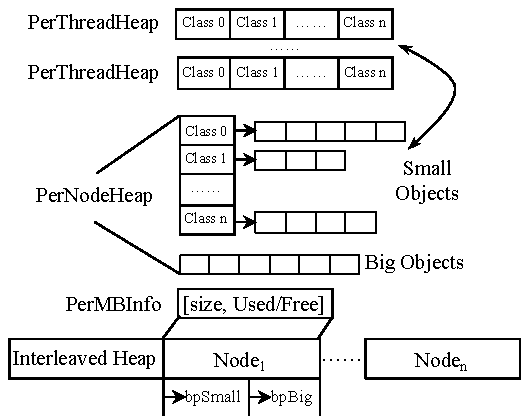
\includegraphics[width=0.45\textwidth]{figure/heaplayout1}
%\includegraphics{figure/overview2}
\end{center}
%\vspace{-0.1in}
\caption{Overview of \NA{}'s Heap Layout.
\label{fig:overview}}
%\vspace{-0.1in}
\end{figure}

As discussed in Section~\ref{sec:intro}, \NM{} proposes an origin-based memory management that should quickly check the origin of every object upon deallocation. In order to support fast checking, \NM{}'s heap layout is designed as  Figure~\ref{fig:overview}. \NM{} requests a large and continuous block of memory from the underlying OS initially, and then divides it evenly into multiple regions based on the number of hardware nodes. Each region is bound to a different physical node via \texttt{mbind} system call. In particular, the first region is bound to the first node, the second one is bound to the second node, and so on. This design enables us to compute the physical node quickly from a memory address: we could compute the index of the physical node by dividing the heap offset by the region size. This layout is different from existing allocators, based on our knowledge. %\todo{There have been machines in the past that use the most significant bits of the physical address to interleave the address space.}

%\NM{} borrows some of these existing mechanisms. First, it uses different mechanisms to manage small and big objects. Second, small objects are also managed by size classes using the BiBOP-style. Third, similar to existing work, such as Linux and TCMalloc~\cite{tcmalloc}, \NA{} utilizes different freelists to track freed objects, and uses the first word of freed objects to link different objects. But the difference of \NM{} is further described in Section~\ref{sec:implement}.

\NM{} also manages small and big objects differently, which is similar to existing allocators as discussed in Section~\ref{sec:commondesign}. Small objects are organized by size classes, and each request will be satisfied from a particular size class. \NA{} utilizes fine-grained size classes for small objects, such as 16 bytes apart for objects less than 128 bytes, and 32 bytes apart for objects between 128 bytes and 256 bytes, then power-of-2 sizes afterward. In \NM{}'s design, big objects are those with a size larger than 512K, which are typically aligned up to megabytes. As shown in Figure~\ref{fig:overview}, each per-node region will be further divided into two sub-regions, one for small objects, and one for big objects. The \texttt{bpSmall} pointer is utilized to track never-allocated small objects, and big ones are tracked with \texttt{bpBig} pointer. 

For small objects, \NM{} utilizes the well-known  ``\textbf{Bi}g-\textbf{B}ag-\textbf{o}f-\textbf{P}ages'' (BiBOP) style that all objects in the same bag (1 MB by default) will have the same size class. Big objects will be always aligned to 1MB. In order to improve the reliability~\cite{FreeGuard, Guarder}, \NM{} tracks the size information and availability information in a separate area (shown as ``PerMBInfo'' of Figure~\ref{fig:overview}): it tracks the size of each size class for small objects, and the size of the big object (aligned to 1 MB) for big objects. This data structure also includes the used/free information for big objects, which allows coalescing multiple continuous big objects into a bigger object upon deallocations. To save space, \NM{} utilizes the lowest significant bit of ``PerMBInfo'' to encode the availability information.

Freed objects of the same size class will be tracked with a freelist. In order to further reduce the contention, \NM{} adapts a per-thread heap that maintains a freelist for each size class, which requires no protection since each thread has its own per-thread heap. However, this may introduce memory blowup~\cite{Hoard} that freed objects of a per-thread heap cannot be utilized for future allocations from other threads, as addressed in Section~\ref{sec:others}. 

%\todo{There is a lot of repetition in the paper.  You mention that you can determine the node from the pointer multple times.}

To support the NUMA architecture, a PerNodeHeap is proposed that has one freelist for each size class and one common freelist for all big objects  from the current node. We will talk about the relationship between per-thread freelist and per-node freelist in Section~\ref{sec:origin}. 

Overall, \NM{} includes a novel layout to quickly compute the physical node (with the memory binding) and a per-node heap to support node-aware allocations. This design allows it to perform origin-based memory management efficiently, as discussed in the next section. 

%mechanisms to re and one per-node freelist for each node to track big objects. \NM{} also maintains per-node freelists to track small objects based on size classes. These freelists are singly linked lists, which uses the first word of every freed object as pointers.  Small freed objects may be migrated between per-thread freelists and per-node freelists, as further described in Section~\ref{sec: others}. 

\subsection{Origin-Based Memory Management} 
\label{sec:origin}

%\todo{In Section III-B, you talk about satisfying allocations from the "un-allocated region" as the last step. Is this memory that is not part of the interleaved heap? It would help to be more clear about what this is. }

As described in Section~\ref{sec:overview}, \NM{} includes an origin-computable design that could quickly determine the origin of each object via the computation. On top of it, we further discuss other aspects of \NM{}'s origin-based memory management as follows.  

First, it includes an origin-based deallocation that will always return a freed object to a freelist with the same origin. In particular, if a freed object is originated from a different node, it is returned to its original node's  freelist. Otherwise, a small object is returned back to the thread's freelist and a big object is returned back to the current node's freelist. Comparing to node-based freelist, there is no need to acquire a lock when operating on the per-thread freelist. Different from all existing work, \NM{} may return a freed object into the per-thread list or its original node's freelist, instead of simply putting into the per-thread list. That is, \NM{} considers the originality of objects for deallocations.   

Second, \NM{} always ensures node-local memory allocations. For small objects, it follows this order: (1) the per-thread's freelist will be checked first, since there is no need to acquire any lock and objects may be still hit in the cache (as they are just accessed by the thread); (2) If the per-thread freelist does not have available objects, \NM{} tries to allocate from the current node's freelist; As mentioned above, a node's freelist holds objects originated from this node. (3) If the last two steps fail,  we will allocate the memory from the current node's un-allocated region, as shown by bpSmall in Figure\ref{fig:overview}. In this way, 
%Since the region is bound to the current node, and objects in the per-thread freelist and the per-node freelist are always originated from the current node, 
\NM{} ensures local allocations for small objects. For big objects, allocation will be satisfied from per-node freelists or un-allocated region (pointed by bpBig pointer in Figure\ref{fig:overview}) of the current node, indicating local allocations for big objects. 

\subsection{Node-Balanced Thread Binding} 
\label{sec:balance}
As described in Section~\ref{sec:intro}, thread migration will cause multiple performance issues for the NUMA architecture. Therefore, \NM{} binds each thread to a node specifically in order to avoid thread migration across different nodes. To improve the balance, \NM{} binds threads to different nodes in an interleaved way so that every node will have a similar number of threads. The first thread will be bound to the node that it is scheduled to run by the OS, and the second thread will be bound to its next node, and so on. Note that \NM{} only binds a thread to a node, instead of a core, which still allows the scheduling initiated by the OS. To perform the binding correctly, \NM{} obtains the hardware topology in the initialization phase via the \texttt{numa\_node\_to\_cpus} API, which tells the relationship between each CPU core and each memory node. Then it intercepts all thread creations in order to bind a newly-created thread to a specific node. In the future, we plan to support user-controlled binding.

%\subsection{Selective Huge Pages} 
%\label{sec:hugepage}

%Based on the existing study~\cite{hugepages}, huge pages can reduce Translation Look-aside Buffer (TLB) misses, since the same size of TLB entries will cover a larger space of memory. However, existing transparent huge page support is not good for the performance~\cite{Gaud:2014:LPM:2643634.2643659, DBLP:conf/asplos/PanwarBG19}, due to hot page effect, page-level false sharing, and increased memory footprint~\cite{DBLP:conf/asplos/MaasAIJMR20}.
 
%\NM{} proposes explicit huge pages to avoid these issues that could always benefit the performance based on our evaluation in Section~\ref{sec:hugepage}. The basic idea of \NM{} is to carefully choose which objects that should be allocated from huge pages: first, shared objects should not be allocated from huge pages, which may introduce page-level false sharing that multiple threads are accessing the same huge page. This will cause unnecessary load imbalance due to concurrent accesses, and remote accesses. Second, if we only utilize partial memory in the same huge pages, then we may waste the remaining memory on the same page. This problem will become more serious for \NM{}'s design, since it is using a big bag (1MB) to hold objects of the same size. 

%If huge pages are only utilized for private objects for threads running on the node, then there is no hot page effect and page-level false sharing. Also, if huge pages are only utilized for big objects that are larger than the page size, then there is no need to worry about unnecessary memory consumption. 
%Based on these observations,  \NM{} only employs huge pages for large objects, with a size larger than 512KB. This design will reduce unnecessary memory waste that only partial pages are actually allocated. Also, \NM{} only employs huge pages for small objects that are predicted to be allocated frequently. For the latter one, \NM{} employs the history information to predict, and only uses huge pages for a size class that has used at least one bag before. Based on our evaluation in Section~\ref{sec:hugepage}, this design balances the performance and memory consumption, which always benefiting the performance. 

%In addition to large objects that has the size larger than the size of a huge page, huge pages are only utilized for small objects that are predicted to be used a lot.  \NA{} employs the history of memory allocation to predict this. 
%Each per-node heap is further divided into two parts as illustrated in Figure~\ref{fig:overview}: small objects will be allocated from the first half and will be allocated using small pages, while big objects will be allocated from the second half with huge pages (2MB). When a big object (with the huge page) is utilized for small objects, only frequently-allocated small objects can utilize such an object. We believe that our design balances the performance and memory consumption.   

\subsection{Interleaved Heap} 

%\todo{In Section III-D, the heuristic to learn private objects from shared objects of the main thread may not always work. What if all allocations happen before children threads are forked, but none are deallocated until after children threads are forked? }

\NA{} proposes an interleaved heap that is inspired by existing profilers\cite{XULIU, MemProf}: many NUMA performances issues are related to shared objects allocated in the main thread. Due to the default first-touch policy~\cite{lameter2013numa, diener2015locality}, objects allocated and touched by the main thread are typically allocated in the node that the main thread is running on. However, these objects can be passed to multiple child threads and be accessed by these threads concurrently so that this node's memory controller becomes the performance bottleneck. 
%causing the load imbalance issue: the memory controller of this node will be concurrently accessed by multiple threads,

To overcome this issue, \NA{} reserves a range of memory for such objects, called ``Interleaved Heap'' as shown in Figure~\ref{fig:overview}. \NA{} utilizes the \texttt{mbind} system call to specify that physical pages of this heap will be allocated from all nodes interleavedly. With this design, when these objects are passed to child threads, these threads may access objects that are allocated from multiple nodes, reducing interconnect congestion and load imbalance of a single node. 

\begin{comment}
\begin{wrapfigure}{r}{0.6\textwidth}
\centering
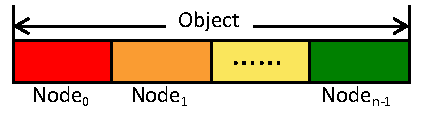
\includegraphics[width=3in]{figure/blockwise}
\vspace{-0.1in}
\caption{Block-wise Memory Allocation\label{fig:blockwise}}
\vspace{-0.1in}
\end{wrapfigure}
\end{comment}

In theory, private objects of the first thread should not be allocated from the interleaved heap, since that will create remote accesses unnecessarily. \NM{} utilizes a simple heuristics to differentiate shared objects from private objects based on allocation callsites: each allocation callsite is treated as a shared one initially, and is allocated from the interleaved heap; Whenever an object is deallocated before creating children threads, indicating such an object is a private one for the main thread, all objects from the corresponding callsite are considered to be private ones, and they are only allocated from the per-node heap afterward. With this heuristics , there is no need to change programs explicitly, although it is more efficient if programmers could provide such information. 

As mentioned above, \NM{} monitors allocation/deallocation pattern of the main thread to identify the share-ability of each callsite. 
%If an allocation callsite is found to be private, then all allocations from this callsite should not allocate from the interleaved heap, but from the normal heap. 
A challenge is to obtain and compare the callsite of each allocation so that we could determine the heap based on the share-ability. In fact, this may introduce high overhead for applications with large amount of allocations, if using the \texttt{backtrace}~\cite{DBLP:conf/icse/SumnerZWZ10, DBLP:conf/cgo/ZengR0AJ014}. For the performance reason, \NA{} utilizes the sum of the stack position and the return address of the allocation invocation to identify a callsite, called ``\textit{callsite key}''. This combination is able to differentiate callsites correctly if an application does not have allocation wrappers, since the stack position can be utilized to identify the function in the stack and the return address tells the invocation placement inside the same function. If a callsite is misidentified, it will not cause any correctness issue, but with some performance penalties/losses. \NA{} utilizes a hash table to track the status of every callsite. 
 % which is fortunately not very expensive given the limited amount of different callsites. 
 
Note that the interleaved heap cannot be achieved by using existing NUMA utilities like \texttt{numactl}. Although \texttt{numactl} could also specify memory allocations to be interleaved. However, \texttt{numactl} could only set the policy for a whole application. Instead, \NM{} only utilizes the interleaved heap for shared objects that are allocated in the main thread, not for all objects. As we evaluated in Section~\ref{sec:interleavedheap}, the interleaved heap is beneficial to the performance for most applications, but not all applications. Therefore, it is better that the interleaved heap is enabled whenever necessary. 

\subsection{Other Mechanisms}
\label{sec:others}

\NM{} also implements the following mechanisms in order to reduce the performance and memory overhead. 

\paragraph{Efficient Object Movement} 
%It is important to reduce memory blowup that freed objects by one thread cannot be utilized by other threads~\cite{Hoard}. 
\NM{} requires to move freed objects between per-thread and per-node freelists frequently. On the one hand, when a per-thread freelist has too many freed objects, some of them should be moved to the per-node freelist so that other threads could re-utilize these freed objects. On the other hand, each per-thread list needs to obtain freed objects from its per-node heap, when a thread is running out of the memory. 

Therefore, an efficient mechanism is required to support frequent movement. A straightforward method is to traverse the freelist to collect a specified number of objects, and then moves all of them at a time to reduce the synchronization overhead. Both TCMalloc and TCMalloc-NUMA utilize this mechanism, which has the following issues: First, traversing a freed object will actually bring its first lines to the cache, since its first word is used as the pointer for the freelist. This traverse will introduce unnecessary cache misses for the current thread, when these objects are moved to other threads later. 
%\NM{} utilizes the first word of each freed object as the pointers for the linked list, where traversing these objects will bring these objects to the cache that the current thread do not need. 
Second, the movement will always move recently-freed objects since they are located in the header of the singly-linked list. However, this is not good for the performance since these recently-freed objects can be still hot in the cache. 
%when moving objects from a per-thread freelist to the per-node freelist, since recently-freed objects can be still hot in the cache. 
%Then a thread will be forced to utilize objects that are not in the cache. 
Third, the traverse of a global freelist may introduce significant lock contention, when multiple threads are moving freed objects from the per-node freelist concurrently. 
%In our Some applications (e.g.,  have been observed a 20\% slowdown due to this straightforward mechanism. %\todo{someone asked where the data come from?} 
 
%\todo{On object migration (section III-E): the authors mention that traversing a freelist will bring cache lines to the traversing thread's cache, causing cache misses for other threads (traversing thread’s cache will be changed). Given that these traversals are reads, this statement seems to be incorrect. The cache coherence mechanism will bring the read cache lines in Shared state, hence their copies in other threads' caches won't be invalidated.}

\begin{figure}[!h]
\centering
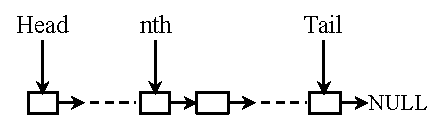
\includegraphics[width=3in]{figure/perthreadlist}
%\vspace{-0.1in}
\caption{Avoiding the traverse of per-thread freelist\label{fig:perthreadlist}}
%\vspace{-0.1in}
\end{figure}

\NM{} proposes an efficient mechanism and special data structures to avoid these issues. First, each per-thread freelist maintains two pointers that point to the least recently used object (shown as the \texttt{Tail} pointer) and the $nth$ object separately (shown as $nth$ in Figure~\ref{fig:perthreadlist}), where the $n$ is a predefined number that is going to be moved. Each freelist also maintains a pointer (\texttt{Header}) pointing to the most recently used object. This structure avoids the traverse of freelist during the movement, and allows the movement of the least recently used objects (between $(n+1)th$ and $Tail$) to the per-node freelist. After the movement, the \texttt{Tail} pointer will be set to the original $nth$ object. 

%\Maintaining the pointer to the $nth$ object requires only a forward traverse to obtain the pointer of $(n-1)th$ object, and then a thread can migrate $n$ objects (between $(n-1)th$ and the \texttt{Tail} object) easily. 
%After the migration,  the \texttt{Tail} pointer can be set to the original $nth$ object. However, this mechanism alone cannot reduce the lock contention when multiple threads are concurrently obtaining objects.

\begin{figure}[!ht]
\centering
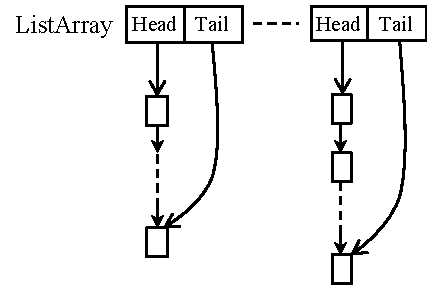
\includegraphics[width=3in]{figure/listarray}
\caption{An array of freelists for per-node heap\label{fig:listarray}}
%\vspace{-0.1in}
\end{figure}

Second, \NM{} also proposes a circular array (``ListArray'' as Figure~\ref{fig:listarray}) that helps move objects from per-node freelist to per-thread freelist. As mentioned above, the per-node freelist could easily become the performance bottleneck, since multiple threads may compete for it concurrently. To address this issue, each per-node freelist is actually consisted of many sub-lists, where a \texttt{Head} pointer and a \texttt{Tail} pointer point to the header and the tail of each sub-list. When a thread is moving multiple objects from the per-node freelist, it could move all objects in a sub-list (pointed by a pair of \texttt{Head} and \texttt{Tail} pointer) at a time. Therefore, there is no need to traverse the whole list to obtain these objects for the movement, which could reduce the contention. 
%Then whenever a thread is migrated object,

%The performance overhead of three types of operations can be greatly reduced with this data structure. First, a remote thread will put a freed object into the freelist, based on the origin-based deallocation. This operation can be done in a constant time, by putting the object into the entry pointed by a \texttt{toPut} pointer. Second, a local thread maybe put multiple objects into it, which can be finished in constant time as well. All objects will be put to the entry pointed by a \texttt{toPut} pointer, and then the pointer will be updated to the next entry. Third, the operations for getting objects from it can be done efficiently by simply moving all objects in the current entry, since there is no need to traverse the freelist. Therefore, this data structure reduces the synchronization issue of all operations. 
%\todo{introduce toPut pointer before using it}
%In order to support the put and get operations to the freelist, this array has two pointers, \texttt{toGetIndex} and  \texttt{toPutIndex}. If a thread tries to obtain freed objects from the per-node heap, it will obtain all  objects pointed by the \texttt{toGetIndex}, and increment the index afterward. If the freelist pointed by the \texttt{toGetIndex} has no freed objects, there is no freed objects in the per-node freelist for this size class.  The put operation will utilize the pointer \texttt{toPutIndex}. There are two scenarios for the put operation. 
%First, 

Note that this array does not increase the overhead of putting objects. If a thread puts a freed object to this array, the object can be placed into the current sub-list in a constant time. Similarly, a freelist could be appended to the current sub-list in a constant time. 
%the object will be placed into the freelist pointed by the \texttt{toPutIndex}, but the index is not updated after the deallocation. Second, when freed objects in a per-thread freelist is above the predefined watermark, the thread will migrate a batch of objects to the freelist pointed by the \texttt{toPutIndex}. After this migration, the current freelist is considered to be full, and will update the index to the next entry in the circular array.

\paragraph{Node-Local Metadata} \NM{} guarantees that all of the metadata is always allocated in the same node, based on its thread binding as described in Section~\ref{sec:balance}. Note that this is only possible under the thread binding. Such metadata includes per-node and per-thread freelists for different size classes, and freelists for big objects. Similarly, \NM{} utilizes the \texttt{mbind} system call to bind the memory to a specific node.  

\paragraph{Reducing Memory Fragmentation When Transparent Huge Pages (THP) is Enabled} When THP is enabled, the OS will prefer to allocate huge pages if a program touches a continuous memory region with the size larger than a huge page (e.g., 2MB). Since \NM{} allocates a large region initially(as shown in Figure~\ref{fig:overview}), huge pages will be allocated correspondingly. Therefore, it is important to reduce memory fragmentation. \NM{} makes multiple threads (from  the same node) share the same memory block, instead of having a separate block for each thread as Scalloc~\cite{Scalloc}. That is, when a thread is running out of the memory, it obtains only multiple objects at a time from the corresponding memory block, typically in the granularity of a page (4KB), instead of getting a whole block (few megabytes) for each per-thread heap. This is the basic reason that \NM{} has much less memory consumption than Scaller, as evaluated in Section~\ref{sec:memory}.  
%Based on our evaluation, this mechanism reduces most of the memory consumption, with the transparent huge page support by default.  

 %every thread has its own freelists for each size class so that there is no need to acquire the lock when an allocation can be satisfied from its per-thread heap, similar to TCMalloc. That is, two threads will not share the same per-thread heap. However, some applications may create new threads after some threads have exited. \NM{} re-utilizes the memory for these exited threads. Basically, \NM{} intercepts thread joins and cancels so that it can assign heaps of exited threads for newly-created threads, and re-utilize their heaps correspondingly.  


%\paragraph{Transparent Huge Page Support:} During the development, we noticed that excessive memory consumption can be imposed when the OS enables transparent huge pages by default. In order to reduce memory consumption, \NM{} makes multiple threads share the same bag (for the same size class), instead of having a separate bag for each thread. If each thread is running out of the memory, it obtains multiple objects at a time from the corresponding bag. Currently, if a class size is less than one page, then we will at most get objects with the total size of one normal page. Otherwise, it will get 4 objects (with the size less than 64 KB) or 2 objects afterward. Based on our evaluation, this mechanism actually reduces the memory consumption for multiple times for a machine with 128 cores and 8 nodes, with the transparent huge page support by default.  

%\paragraph{Cache Warmup} \NM{} also borrows the cache warmup mechanism of TCMalloc~\cite{tcmalloc}: it will insert all objects in a page into the freelists, if there is no objects in the per-thread freelist. We believe that inserting multiple objects into the freelist will benefit data prefetches, since the insertion is a simple and predictable pattern. With this mechanism, \texttt{raytrace} improves the performance by 10\%. However, this is the only application that we observed such performance improvement. There is no impact on other applications. 

%TCMalloc utilizes a \texttt{mmap} system call to obtain multiple pages (depending on the class size) from the OS each time, when it is running out of the memory for one size class. For such a memory block, TCMalloc inserts all objects of this block into its central freelist at one time. Since TCMalloc utilizes the first word of each object as the pointer for the freelist, this mechanism warms up the cache by referencing the first word of each object during the insertion. According to our observation, this warmup mechanism improves the performance of one application (\texttt{raytrace}) by 10\%. Based on our understanding, the performance improvement is caused by data prefetches, since inserting objects to the freelist has a simple and predictable pattern. \NM{} employs a similar mechanism for small objects with the size less than 256 bytes, and adds all objects inside a page to the per-thread freelist. 

%we propose the combination of per-node heap and per-thread cache. In order to reduce the contention, \NM{} will obtain multiple objects at a time from the per-node heap. 

 
%https://queue.acm.org/detail.cfm?id=2852078


\section{Experimental Evaluation}
\label{sec:evaluation}

This section aims to answer the following research questions: 

\begin{itemize}
\item \textbf{Performance:} How is \NM{}'s performance, comparing to popular allocators and NUMA-aware allocators? (Section~\ref{sec:performance}) 
\item \textbf{Memory Consumption:} What is the memory consumption of \NM{}? (Section~\ref{sec:memory})
\item \textbf{Scalability:} How is the scalability of \NM{}? (Section~\ref{sec:scale})
\item \textbf{Impact of Design Choices:} How important every design choice can actually impact performance? (Section~\ref{sec:design})	
\end{itemize}

\begin{comment}

\begin{table}[!ht]
 \centering
   \caption{Machine specifications for evaluation
   \label{table:Machine}}
  %\setlength{\tabcolsep}{1.0em}
\begin{tabular}{l | l }
\hline
Category & Information \\ \hline
CPUs/Model 	& Xeon(R) Platinum 8153\\ \hline
CPU Frequency & 2.00GHz\\ \hline
NUMA Nodes  & 8 \\ \hline
Physical Cores  & 8$\times$16 \\ \hline
Node Latency &  \specialcell{local: 1.0 \\ 1 hop: 2.1 \\ 2 hops: 3.1}\\ \hline
Interconnect Bandwidth  & 10.4GT/s\\ \hline
Linux & Debian 10\\ \hline
Compiler &  GCC-8.3.0 \\ \hline
%Memory Bandwidth & 19.87 GB/s & \\ \hline
  \end{tabular}
  %\vspace{-0.4in}
\end{table}
\end{comment}

\textbf{Experimental Setup:}  \NM{} was evaluated on a Intel Xeon(R) Platinum 8153 machine with 8 nodes, where each node has 16 cores. Any two nodes are less than or equal to 3 hops, where the latency of two hops and three hops is 2.1 and 3.1 separately if the latency of local accesses is 1.0. The machine is installed with 512GB memory. The underlying OS is Linux Debian 10 and the compiler is GCC-8.3.0. For the evaluation, the hyperthreading was turned off, but both transparent page support and AutoNUMA are  enabled. The performance data shown in this paper is the average of 10 runs, in order to avoid any bias caused by unexpected events.  

\begin{comment}
\begin{table}[!ht]
 \centering
  %\setlength{\tabcolsep}{1.0em}
\begin{tabular}{c | c | c}
\hline
System & \textbf{Machine A} & \textbf{Machine B} \\ \hline
CPUs/Model & Xeon Gold 6138	& Xeon(R) Platinum 8153\\ \hline
CPU Frequency & 2.10GHz & 2.00GHz\\ \hline
NUMA Nodes & 2 & 8 \\ \hline
Physical Cores & 2$\times$20 & 8$\times$16 \\ \hline
Node Latency & \specialcell{local: 1.0 \\ 1 hop: 2.1} & \specialcell{local: 1.0 \\ 1 hop: 2.1 \\ 2 hops: 3.1}\\ \hline
Interconnect Bandwidth & 8GT/s & 10.4GT/s\\ \hline
Linux & Ubuntu 18.04 & Debian 10\\ \hline
Compiler & GCC-7.5.0 & GCC-8.3.0 \\ \hline
%Memory Bandwidth & 19.87 GB/s & \\ \hline
  \end{tabular}
   \caption{Machine specifications for evaluation
   \label{table:Machine}}
  %\vspace{-0.4in}
\end{table}

\end{comment}

\subsection{Performance Evaluation}

\label{sec:performance}
\begin{figure*}[!ht]
    \centering

    \includegraphics[width=7in]{figure/8-node-parsec-perf.jpg}
    \caption{Performance of different allocators, where all data is normalized to \\ that of the default Linux allocator. Here, a lower bar indicates a better performance.
    \label{fig:perf}}
 \end{figure*}
 
 \todo{What is the issue of freqmine? Maybe we should add this application.} 
 
 We compare \NM{} with multiple popular allocators, such as the default Linux allocator, TCMalloc-2.7~\cite{tcmalloc},  TCMalloc-NUMA~\cite{tcmallocnew}, jemalloc-5.2.1~\cite{jemalloc}, Intel TBB--2020.1~\cite{tbb}, Scalloc-1.0.0~\cite{Scalloc}, and mimalloc~\cite{mimalloc}. Among them, TCMalloc, jemalloc, TBB, and mimalloc are commercial allocators designed and maintained by Industrial Giants, like Google, Facebook, Intel, and Microsoft separately. We do not include Hoard~\cite{Hoard} as it is not the state-of-art anymore~\cite{Scalloc, mimalloc}. Multithreaded applications chosen to evaluate the performance include PARSEC applications~\cite{parsec}, and seven real applications like \texttt{Apache httpd-2.4.35}, \texttt{MySQL-5.7.15}, \texttt{Memcached-1.4.25}, \texttt{SQLite-3.12.0}, \texttt{Aget}, \texttt{Pfscan}, and \texttt{Pbzip2}. For the performance evaluation, we utilize 128 threads, which is the same as the number of cores of the evaluated machine. Note that we currently have an issue to run freqmine, an openmp application, which is excluded right now. 
 
PARSEC applications are using native inputs~\cite{parsec}. For \texttt{MySQL}, we use \texttt{sysbench} with 128 threads separately, each issuing 100,000 requests. The \texttt{python-memcached} script is used to exercise \texttt{Memcached}, with 3000 loops to get the sufficient runtime~\cite{memcached}. The \texttt{ab} is used to test \texttt{Apache} server~\cite{apachetest}, by sending 1,000,000 requests in total. \texttt{Aget} is tested by downloading a 30-MB file, and \texttt{Pfscan} is tested by searching  a keyword in a 500MB data. In terms of \texttt{Pbzip2}, we test it by compressing 10 files with 30MB each. Finally, \texttt{SQLite} is tested through a program called \texttt{threadtest3}~\cite{sqlitetest}. 

%\todo{The number of threads of all benchmarks were adjusted according how many cores and nodes in the target machine to make threads could be properly distributed over the nodes and cores, making the number of threads as close as the number of cores. In the test machine, the thread number is 128.}

%In the Hoard~\cite{Hoard} benchmarks, we used 100 iterations and 1,280,000 64-byte objects for threadtest and also we run larson for 10 seconds with 1,000 7-2048 bytes object to cover all size classes in almost all allocators for 10,000 iterations.For false sharing , we used 100,000 inner-loop , 100,000 iterations with 8 bytes objects. 

%The number of threads of all benchmarks were adjusted according how many cores and nodes in the target machine to make threads could be properly distributed over the nodes and cores, making the number of threads as close as the number of cores. Mostly, thread number was 40 in the Machine A and 128 in the Machine B, and I will give the specific number below if it is not this default value. 

The performance results are shown in Figure~\ref{fig:perf}, where the runtime of each allocator is normalized to that of Linux's default one. \textit{\NM{} is configured with the interleaved heap support for most applications, except for \texttt{canneal} and \texttt{raytrace}}. As further discussed in Section~\ref{sec:interleavedheap}, the interleaved heap may have a harmful performance impact for the serial phases, as it turns some local accesses to remote ones. %Therefore, the data of \texttt{canneal} and \texttt{raytrace} are collected without the interleaved heap. 
We believe that this option is acceptable, since users could determine easily whether they should disable the interleaved heap: if an application has a large portion in the serial phase, then the interleaved heap should be disabled. 
%The impact of the interleaved heap is further discussed and evaluated in Section~\ref{sec:interleavedheap}. 
 %With the interleaved heap,  allocations from the main thread can be satisfied in remote NUMA nodes, this design may lead to a large number of remote accesses for the serial phase. since both of them spend a large portion of their time (over 62\% and 82\%) in the serial phase (before creating any child thread),
 %These two figures show the best data for these two applications, without the support of the interleaved heap.    




Overall, \NM{} has the best performance among these allocators. \NM{} is running 18.5\% faster than the default allocator, and 15.8\% faster than the second-best one--TCMalloc~\cite{tcmalloc}, but does not run significantly slower than other allocators in almost all evaluated applications. For the best case (e.g., \texttt{fluidanimate}), \NM{} is running up to $6.4\times$ faster than the default Linux allocator, and it is $4.6\times$ than the second-best one--TCMalloc.  Comparing with the NUMA-aware allocator -- TCMalloc-NUMA~\cite{tcmallocnew}, \NM{} runs 23\% faster. The default Linux allocator achieves good performance on the NUMA architecture due to its arena-based design, where each freed object will be returned back to its original arena.
This design is integrating well with Linux's first-touch allocation policy~\cite{Lameter:2013:NO:2508834.2513149} to ensure most thread-local allocations. 
In contrast, other allocators typically utilize a per-thread cache to store objects that are deallocated by the current thread, which may lead to remote accesses as described in Section~\ref{sec:intro}.  TCMalloc-NUMA and mimalloc are two allocators that are claimed to support the NUMA architecture among them~\cite{tcmallocnew}. But TCMalloc-NUMA's performance is even worse than that of TCMalloc. Based on our understanding, TCMalloc-NUMA is based on TCMalloc-0.97 (released in 2008), which does not have new features of TCMalloc-2.7 (the version for our evaluation). mimalloc only has the very basic NUMA support, which is the reason why it is not performing as well as \NM{}.  


Figure~\ref{fig:perf} shows that \NM{} has a similar or better performance than the default allocator in almost every application. Further, \NM{} has a significant performance improvement (over 20\%) in the following applications, including \texttt{canneal}, \texttt{dedup}, \texttt{fluidanimate}, \texttt{streamcluster}, and \texttt{pbzip2}. Among them, \NM{} has a super performance for \texttt{fluidanimate}, due to the following reasons. First, the interleaved heap contributes to $3.23\times$ performance speedup, as shown in Figure~\ref{fig:interleavedheap}. Second, node-balanced thread binding improves the performance by over $4\times$. 

\textbf{Confirming the number of remote accesses:} We further examine the number of remote accesses to confirm whether \NM{} significantly reduces them due to its design. We utilize the \texttt{perf} to collect the number of remote accesses (both load and store) on these applications when they are running with all allocators. 
%In our machine, we can collect these numbers using the following command: \texttt{perf stat -e node-load-misses,node-store-misses,dTLB-store-misses,dTLB-load-misses} 

The results are shown in Figure~\ref{fig:remoteAccess}. We combine the performance (shown as bars) and remote accesses (red lines) together for a better comparison. We only use five applications that \NM{} has significantly better performance than other allocators.  For three applications, such as \texttt{dedup}, \texttt{fluidanimate}, and \texttt{streamcluster}, \NM{}  significantly reduces the number of remote accesses, comparing to other allocators. That is the reason why it has much better performance on these applications. Let us utilize \texttt{fluidanimate} as an example. TCMalloc and the default Linux allocator has  $5.2\times$ and $5.4\times$ remote accesses than \NM{}. This explains why \NM{} is running up to $6.4\times$ faster than the default Linux allocator, and  $4.6\times$ than the second-best one--TCMalloc. 

However, there is no much difference on the number of remote accesses for \texttt{canneal} and \texttt{dedup} compared with other allocators. Based on our investigation, \NM{} is running faster than others due to the usage of huge pages. When transparent huge page support is enabled, \NM{} utilizes huge pages instead of small pages. Therefore, \NM{} has much less TLB misses, due to the use of huge pages. For example, for \texttt{canneal}, \NM{}'s TLB misses is 452 $times$ lower than that of \texttt{glibc}.

%data in https://docs.google.com/spreadsheets/d/1WqWH5J7CcQuV8Vs4HnqRSC7TZpgQGPB9Gh2knHPSZPU/edit?usp=sharing

%We also observe some similar results for other applications. For \texttt{dedup}, the \texttt{glibc} allocator introduces 17850 time more TLB misses than \NM{}. Note that we only collect these two factors here, where the performance of allocators can be caused by other reasons, such as memory management operations.  


\begin{figure}[!h]
    \centering
    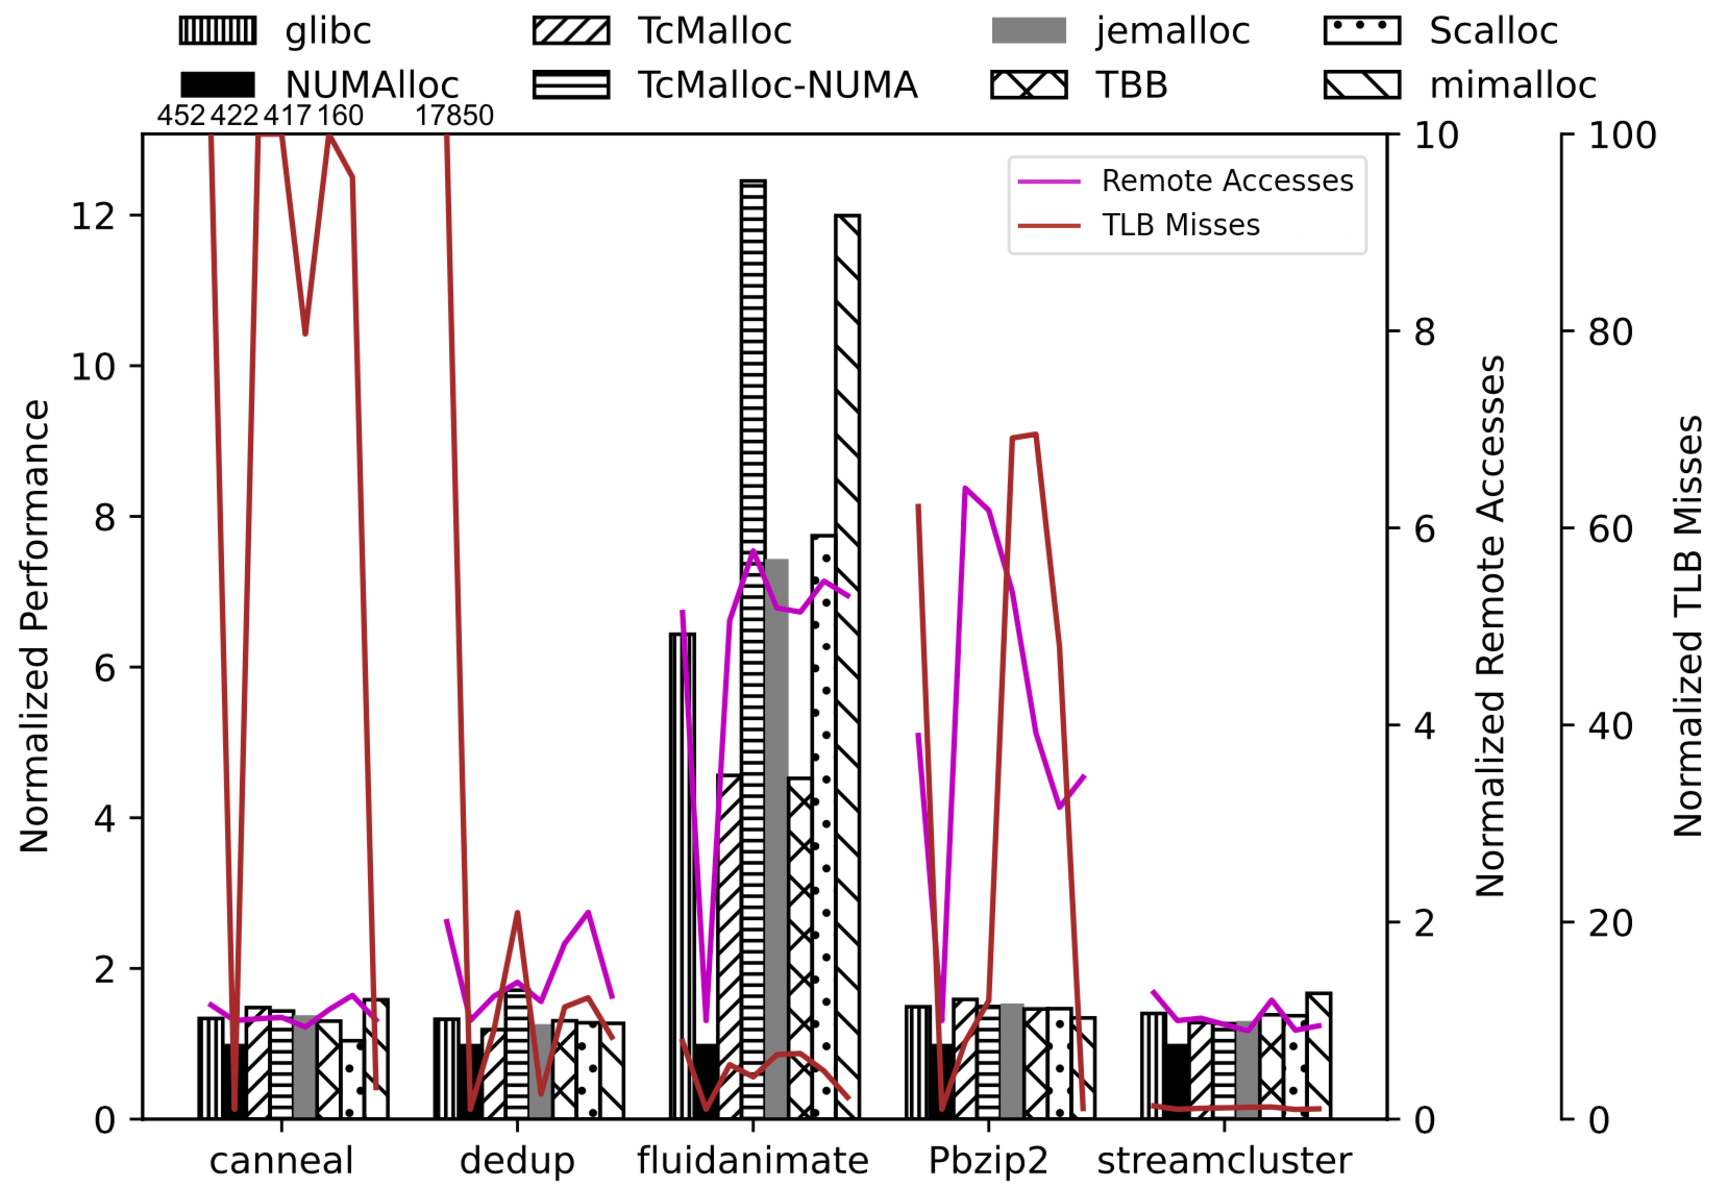
\includegraphics[width=3.5in]{figure/remote-access.pdf}
    \caption{Normalized runtime and the number of remote accesses of different allocators, where all of them are normalized to \NM{}. }
    \label{fig:remoteAccess}
\end{figure}
%\todo{Change "Performance" to runtime, also change the the performance/remote accesses" scale to 8, maybe put NUMAlloc to the first, change TcMalloc to TCMalloc. }

Based on our understanding, \NM{}'s big reduction of remote accesses can be attributed to the following factors: (1) region-based memory allocation that ensures local allocation; (2) (Node-balanced) thread binding; (3) Node-local meta data. 
%Further, \NM{} allocates a large chunk of memory initially, then the OS tends to utilize huge pages if possible, although this mechanism may introduce more memory consumption as evaluated in Section~\ref{sec:memory}.  

\begin{comment}
\begin{table}[htp]
    \centering
    \footnotesize
    \begin{tabular}{l|c| c|c|c|c|c|c|c|c}
    \multicolumn{2}{c|}{Application} & glibc & \NM{} & TCM & TCM-NUMA & jemalloc & TBB & Scalloc & mimalloc \\ \hline
    \multirow{2}{*}{canneal} & Remote & 772 & 613 & 718   & 626 & 690 & 752 & 655 & 709\\ \cline{2-10}
    & TLB Misses &  & 975  &    &  &1876  & 1910 & 1836 & 1876 \\ \hline
    \multirow{2}{*}{dedup}  & Remote & 35.7 & 23.8 & 23.2 & 32.6 & & 29.9 & 28.4 & 23.7\\ \cline{2-10}
     & TLB &  & 21.6 &    &  & & 31.1 & 42.0  & 19.2\\ \hline
    \multirow{2}{*}{fluidanimate} & Remote  & 784 & 145 & 755 & 902 & & 741 & 798 & 749\\ \cline{2-10}
    5.2
   & TLB  &  & 11.9  &    &  & & 116 & 137 & 100\\ \hline
    \multirow{2}{*}{streamcluster} & Remote  & 762 & 571 & 602 & 548 & & 768 & 497 & 570\\ \cline{2-10}
    &  TLB  &  & 12.1 &    &  & & 1455 & 1410 &  1432\\ \hline
    \multirow{2}{*}{pbzip2} & Remote  &  59.3 & 15.2 & 102 & 98.8 & & 62.5 & 45.8 & 60.4\\ \cline{2-10}
    & TLB &  & 0.8 &    &  & & 98.1 & 66.8 & 26.7 \\ \hline
    \end{tabular}
    \caption{TLB misses when using different allocators. The data shown is mega. }
    \label{tab:characteristics}
\end{table}

\end{comment}

%Table~\ref{tab:characteristics} shows that \NM{} significantly reduces the number of remote accesses and TLB misses due to its region-based design. 

%\todo{Hanmei: maybe we need to get the data on these applications. perf stat -e node-loads, node-load-misses, node-stores, node-store-misses ./APP a.out}



%We  can see that the average value of \NM{} is 0.97 in Machine A and 0.92 in Machine B and it is always the best among all other allocators. The reason that \NM{} got better performance in Machine B is that there are more nodes and more cores in Machine B, which means \NM{} could be very helpful to better to take use hardware resource of multi nodes and cores. but we could get amazing improvement if we shutdown interleaved heap in \NM{} and we will give the data in following sections.In the figure ~\ref{8node-parsec-perf}, we could see more exciting improvement from \NM{}, with average normalized value of 0.92 that is not only the best but also far aware better than all the rest allocators that TCMalloc and jemalloc got 0.99, TCMalloc-NUMA and TBB got roughly 1.07 and 1.01 separately. And also, we can see that the performance of \NM{} is the best for almost each single applications, especially it got 0.17 in fluidanimate and 0.66 in streamcluster which is far better than any of other allocators. As the same thing, the performance of ratrace and canneal is not good here, we will talk about it later after we shut down the interleaved heap.


%In the figure ~\ref{hoard-perf}, we show the normalized performance for Hoard benchmarks in Machine A and Machine B separately. We can see from figure ~\ref{hoard-perf} that the average value of \NM{} is also the best, which is 0.47 that means 2 times faster than default Linux Allocator, and jemalloc got 0.7 and Scalloc got 0.9. In the threadtest, the normalized value of \NM{} is 0.19 , far better than any of others, which means there are few central free list competitions, mainly contributed by properly node management and low overheads operations. For false sharing, \NM{}'s performance is also almost the best as same as Scalloc and jemalloc, which means they could handle false sharing issues very properly. In the larson, \NM{} and TCMalloc are the best, which mainly contributed by their low overheads for allocation and remote de-allocation, but due to our better node management, \NM{} could be better in the Machine B which will be mentioned later. In the figure ~\ref{hoard-perf}, we can also see that \NM{} got lowest average normalized value:0.33, significantly smaller than any of others that TBB got 0.99, Scalloc and jemalloc got roughly 1.14. And also, \NM{} and Scalloc could handle false sharing issue very well, and \NM{} could extremely well reduce central free list competition in threadtest. In larson, \NM{} is the best due to its properly multi-node management. 


\subsection{Memory Consumption}
\label{sec:memory}

We also measure the maximum memory consumption of these allocators. For non-server applications, such as \texttt{Aget}, \texttt{Pbscanf}, \texttt{Pbzip2} and all PARSEC applications, we utilized the sum of the \texttt{maxresident} output from the \texttt{time} utility and the size of huge pages, since the \texttt{time }output does not include huge pages. 
To determine the size of huge pages, a script is used to periodically collect the number of huge pages by reading from \texttt{/proc/meminfo} file, and then the maximum value of huge pages is used. 
For server applications, such as \texttt{MySQL}, \texttt{SQLite}, and \texttt{Memcached}, \texttt{Apache}, the maximum memory is collected by the sum of both \texttt{VmHWM} and \texttt{HugetlbPages} fields from \texttt{/proc/PID/status} file, after the corresponding client exits. 
%We always reboot server applications for each single test. 

%\end{comment}

% %\renewcommand{\arraystretch}{1.5}
\begin{table}[tp]
\footnotesize
	\setlength{\tabcolsep}{0.3em}
  \centering
    \begin{tabular}{|l|r|r|r|r|r|r|r|}
    \hline
    \multirow{2}{*}{Apps}&
    \multicolumn{7}{c|}{Memory Usage (MB)}\\
    \cline{2-8}
    &Linux&\NM{}&TcM&TcM-N&jem&TBB&Scalloc \\ \hline
    \hline
    blackscholes&615&509&621&623&633&615&630\\ \hline
    bodytrack&37&161&45&46&570&37&1994\\ \hline
    canneal&888&879&774&757&1294&888&36149\\ \hline
    dedup&912&1236&983&1023&1389&912&8556\\ \hline
    facesim&560&500&603&601&1133&547&3056\\ \hline
    ferret&184&493&195&183&596&184&3377\\ \hline
    fluidanimate&470&392&483&484&481&470&3437\\ \hline
    raytrace&1288&1472&1092&1543&1287&1288&4398\\ \hline
    streamcluster&113&105&123&121&127&113&193\\ \hline
    swaptions&33&268&16&21&540&37&1817\\ \hline
    vips&228&536&248&269&778&227&3681\\ \hline
    x264&2859&2721&3047&3064&3719&2859&5402\\ \hline \hline  
    Aget&8&74&11&10&93&8&80 \\ \hline
    Apache&8&34&10&9&10&4&42\\ \hline
    Memcached&16&80&25&24&41&18&263\\ \hline
    Mysql&277&732&314&315&500&276& N/A \\ \hline
    Pbzip2&463&747&817&813&1121&454&4881 \\ \hline
    Pfscan&522&542&528&528&535&522&554\\ \hline
    Sqlite3&45&284&60&75&139&44&681 \\ \hline
    \hline
    Total&{\bf 9527}&{\bf 11763}&{\bf 9993}&{\bf 10510}&{\bf 14986}&{\bf 9502}&{\bf 79190}\cr\hline
    \end{tabular}
  \caption{Memory consumption of different allocators. Here, TcM stands for TcMalloc, TcM-N is TcMalloc-NUMA, and jem is jemalloc. \label{tab:memory_consumption}}
\end{table}


Memory overhead is listed in Table~\ref{tab:memory_consumption}. In total, \NM{}'s memory consumption is around 45\% more than that of the default Linux allocator, but it is better than \texttt{jemalloc} and  \texttt{mimalloc}, and is $6\times$ better than \texttt{scalloc}.  Overall, the \texttt{glibc} allocator has the smallest memory consumption, and TCMalloc is the second-best one. 
%Scalloc is the worst one in terms of memory consumption, which consumes around  $8.3\times$ more memory that that of TBB.  
 
\NM{}'s more memory consumption is mainly due to the following reasons. \NM{} allocates a large memory block from the OS. When transparent huge page support is enabled, then all memory will be allocated from huge pages. The same reason also applies to Scalloc, which also allocates a continuous huge region of virtual memory from the underlying OS initially. Comparing to Scalloc, \NM{} makes all threads share the same bag for each size class, as described in Section~\ref{sec:others}, which effectively reduces its memory consumption by multiple times. In comparison, Scalloc utilizes $6\times$ more memory when transparent huge page support is enabled.  

We further confirmed the memory consumption when transparent huge page support is disabled, which can be seen in Table~\ref{tab:memory_consumption}. Comparing to the default glibc allocator, \NM{}'s total memory overhead is around 10\%, with the GEOMEAN of 5.6\% only. The total memory consumption is decreased from 16878 MB to 12801 MB,  when transparent huge pages are disabled. Other allocators will not be affected much by transparent huge pages, since they typically obtain a small chunk from the OS each time, less than the size of a huge page (2MB), then the OS will not allocate physical pages from huge pages by default.  
Therefore, we believe that \NM{}'s memory consumption is acceptable. 

%Second, \NM{} may not return the memory to the OS immediately for large pages. However, we believe that its memory consumption is acceptable. 
  %which actually shows the worst case for \NM{}. The OS will utilize huge pages if a memory area is larger than the size of a huge page (2MB). Since \NM{} utilizes \texttt{mmap} to allocate a huge chunk of virtual memory, this makes all heap memory for real objects will be allocated from huge pages. Currently, \NM{} also utilizes 1MB as the superblock for each size class, making objects of a size class that will occupy at least 1MB even if it only uses an object inside. 
 % Therefore, an application with many size classes will waste more memory. \NM{} makes all threads share the same bag for each size class, as described in Section~\ref{sec: others}, which effectively reduces its memory consumption by multiple times. 
 
 %Scalloc has excessive memory consumption, since its design does not support transparent huge pages very well. Similar to \NM{}, Scalloc utilizes a \texttt{mmap} system call to allocate a continuous huge region of virtual memory from the underlying OS. Since every thread will get a virtual span (2MB) for each size class in Scalloc, it will utilize 2MB physical memory even if only a word is touched. Differently, \NM{} avoids this issue as described in Section~\ref{sec: others}.
% the OS will assign a huge page when transparent huge page is enabled by default. Thus, if only one object is allocated from a size class, 
 
%\renewcommand{\arraystretch}{1.5}
\begin{table}[tp]
\footnotesize
	\setlength{\tabcolsep}{0.3em}
  \centering
    \begin{tabular}{|l|r|r|r|r|r|r|r|}
    \hline
    \multirow{2}{*}{Apps}&
    \multicolumn{7}{c|}{Memory Usage (MB)}\\
    \cline{2-8}
    &Linux&\NM{}&TcM&TcM-N&jem&TBB&Scalloc \\ \hline
    \hline
    blackscholes&615&509&621&623&633&615&630\\ \hline
    bodytrack&37&161&45&46&570&37&1994\\ \hline
    canneal&888&879&774&757&1294&888&36149\\ \hline
    dedup&912&1236&983&1023&1389&912&8556\\ \hline
    facesim&560&500&603&601&1133&547&3056\\ \hline
    ferret&184&493&195&183&596&184&3377\\ \hline
    fluidanimate&470&392&483&484&481&470&3437\\ \hline
    raytrace&1288&1472&1092&1543&1287&1288&4398\\ \hline
    streamcluster&113&105&123&121&127&113&193\\ \hline
    swaptions&33&268&16&21&540&37&1817\\ \hline
    vips&228&536&248&269&778&227&3681\\ \hline
    x264&2859&2721&3047&3064&3719&2859&5402\\ \hline \hline  
    Aget&8&74&11&10&93&8&80 \\ \hline
    Apache&8&34&10&9&10&4&42\\ \hline
    Memcached&16&80&25&24&41&18&263\\ \hline
    Mysql&277&732&314&315&500&276& N/A \\ \hline
    Pbzip2&463&747&817&813&1121&454&4881 \\ \hline
    Pfscan&522&542&528&528&535&522&554\\ \hline
    Sqlite3&45&284&60&75&139&44&681 \\ \hline
    \hline
    Total&{\bf 9527}&{\bf 11763}&{\bf 9993}&{\bf 10510}&{\bf 14986}&{\bf 9502}&{\bf 79190}\cr\hline
    \end{tabular}
  \caption{Memory consumption of different allocators. Here, TcM stands for TcMalloc, TcM-N is TcMalloc-NUMA, and jem is jemalloc. \label{tab:memory_consumption}}
\end{table}

 
\begin{comment}


In Figure~\ref{2node-hoard-mem}, the average normalized value of \NM{} is larger than others, but actually not too much, which is 2.3 for \NM{}, 1.9 for TCMalloc-NUMA and 1.8 for TCMalloc. It is because that proper node management is utilized in \NM{} and also in TCMalloc-NUMA, so that each node also preserves some memory not only thread locals. But we believe that these little more memory overheads are totally acceptable. It is also the same thing for Figure 10, that the average value for \NM{} is a little higher than others, which is 5.3. But in this 8 nodes machine, \NM{} is not the worst, that Scalloc's average value is 25 and jemalloc is 9.4. One main reason that the value of \NM{} is smaller is that we use mini-size bags in \NM{} which is less than the size of one page for small objects and also memories for small objects are shared per node but per cores in Scalloc.
	
\end{comment}


\subsection{Scalability}
\label{sec:scale}

We also evaluated the scalability of different allocators. We do not use the same applications in Section~\ref{sec:performance}, as they are not scalable by design. We have verified blacksholes, bodytrack, canneal, and raytrace. For instance, raytrace has not performance different when running with 16 threads or 40 threads. Therefore, we are using four synthetic applications from Hoard~\cite{Hoard}, including \texttt{threadtest}, \texttt{larson}~\cite{Larson}, \texttt{cache-scratch} and \texttt{cache-slash}, which is also employed by existing work~\cite{Scalloc}. \texttt{larson} simulates a multithreaded server that could respond to requests from different clients, and \texttt{threadtest} is an application that performs a large number of allocations and deallocations within a specified number of threads. Both \texttt{cache-scratch} and \texttt{cache-thrash} tests false sharing issue that can be introduced by allocators, where  multiple threads are getting and accessing different objects in the same cache line. 
%Passive false sharing is introduced upon deallocations, where a freed object can be utilized by another thread. In contrast, active false sharing is introduced during the initial allocations, where multiple continuous objects sharing the same cache line are allocated to different threads. The synthetic applications have a better scalability by design than other evaluated applications in the last section. 
%Since other allocators cannot specify the configuration, we only evaluate the scalability with different number of threads. 

In the evaluation, we maximize the number of threads on each node for \NM{}. For instance, the result of 32 threads will use 2 nodes, as each node has 16 cores. For other allocators, we only specify the number of threads, and it is up to the OS to perform the scheduling. The corresponding data is shown in Figure~\ref{sythentic-scalability}. All data are normalized to the data of one thread of the Linux's default allocator, where the higher is better.  

\begin{figure*}[!th]
    \centering
    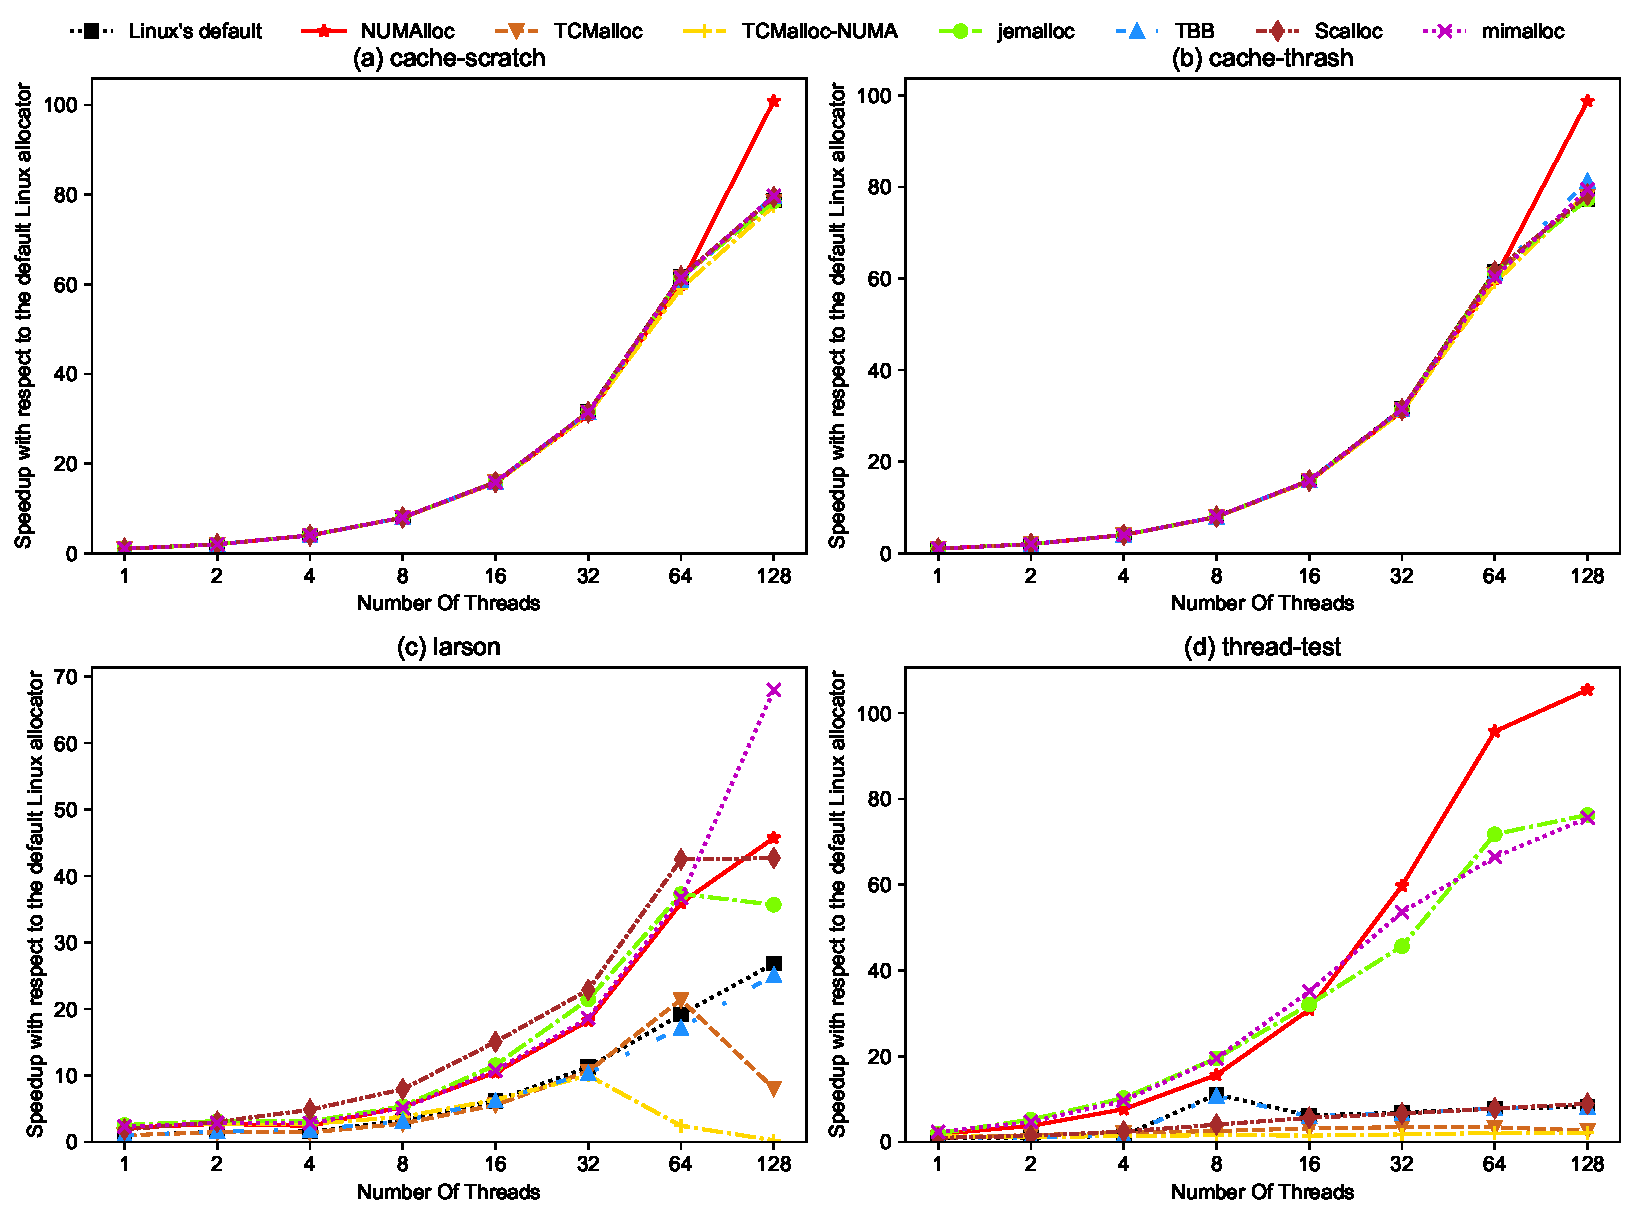
\includegraphics[width=\textwidth]{figure/sythentic-scalobility-new.pdf}
    \caption{Scalability evaluation of different allocators.\\ All data is normalized to the runtime of the default Linux allocator with one thread.}
    \label{sythentic-scalability}
\end{figure*}

Overall, \NM{} has the best performance when the number of cores is 128. Its average speedup is $81\times$, comparing to Linux's allocator with one thread, while the second-best allocator--\texttt{mimalloc}-- has $72\times$ speedup. In contrast, the default Linux allocator only has the speedup of $49\times$. That is, \NM{} has the best scalability. When computing the speedup using the data of one thread of each allocator, \NM{}'s average speedup is $65\times$, while the second-best one is $54\times$. All of these data indicate that \NM{} is scalable to 128 cores. \NM{} only perform worse than mimalloc for larson with 128 threads, but it performs better for other applications. We don't know the exact reason of this.  


%Among these applications, \texttt{cache-scratch} tests passive false sharing, and \texttt{cache-thrash} tests active false sharing. False sharing occurs when multiple threads are concurrently accessing different words in the same cache line. 
%Passive false sharing is introduced upon deallocations, where a freed object can be utilized by another thread. In contrast, active false sharing is introduced during the initial allocations, where multiple continuous objects sharing the same cache line are allocated to different threads. 
%For these false sharing tests, we use 100,000 inner-loop, and 100,000 iterations with 8-byte objects.
TCMalloc has serious issues of both active and passive false sharing issues, which is the major reason that it does not perform well on both \texttt{cache-scratch} and \texttt{cache-thrash}. 
\NM{} will not introduce active false sharing, since each thread will get a page of objects initially. Although \NM{} might introduce passive false sharing due to its per-thread cache design, it avoids remote allocations across the node. 
%We believe that is the major reason for its better performance. Other allocators do not have such mechanisms. That is the reason why 
 \NM{} is one of the best allocators for \texttt{cache-scratch}, and achieves much better speedup than all other allocators in \texttt{cache-thrash} (30\% faster than the second-best one), as shown in Figure~\ref{sythentic-scalability}. 
 
 %\texttt{larson} is to simulate a multithreaded server that could respond to requests from different clients. \NM{} is around 16\% faster than the second-best allocator--TCMalloc.   \texttt{threadtest} is an application that performs a large number of allocations and deallocations within a specified number of threads. \NM{} is $2.6\times$ faster than the second-best one (jemalloc), when there are 128 threads.
 %Each thread will receive a random number of objects in the beginning, perform a random number of allocation and deallocations to simulate the handler for processing requests, and then pass objects to the next thread. We test \texttt{larson} for 10 seconds with 1,000 objects for 10,000 iterations, where each allocation is between 7 bytes and 2048 bytes. 
 %As shown in Fig.~\ref{sythentic-scalability},  



%Also, it allows to specify how much work to be done between each allocation and deallocation. For \texttt{threadtest}, we use 100 iterations, 1,280,000 allocations, 0 work, and 64-byte objects (for the allocation).  This benchmark will stressfully test the performance overhead of allocation and deallocation. For this application, 
 %since every thread will has its own heap and it only imposes some when getting objects from the shared bag. But \NM{} obtains a number of objects at a time, at the page level, which significant reduce the possibility of contention. 


%On average,  \NM{} is running 79\% faster than the second-best one (Scalloc), and $2.2\times$ faster than the default Linux allocator. Multiple reasons contribute to the good performance of \NM{}: \NM{} imposes very minimal system call overhead, and little synchronization overhead. Also, it introduces less remote accesses than all other allocators, due to its NUMA-aware design. Other allocators have more or less false sharing issue, or incurs remote accesses.  
%\todo{Surprisingly, TCMalloc and  }.



%That is the reason why it has a good performance as the Linux allocator for \texttt{cache-thrash}.

 
\begin{comment}

\begin{figure}[!ht]
    \centering
    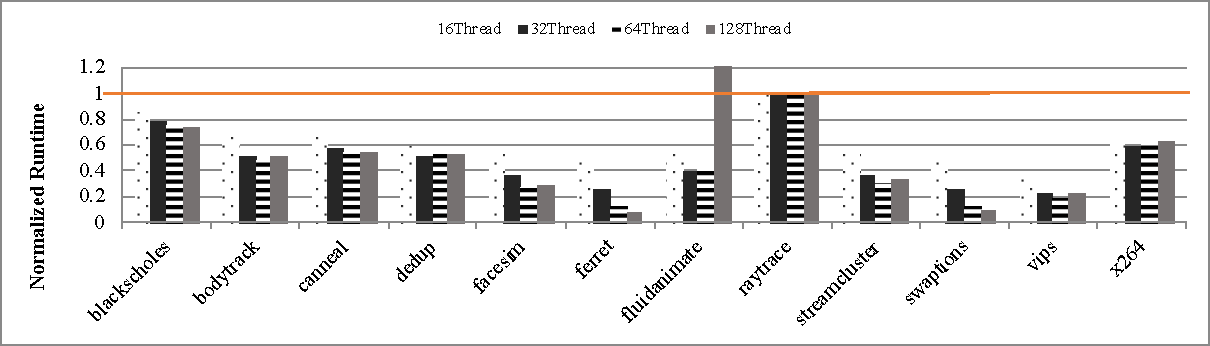
\includegraphics[width=5.5in]{figure/scalobility-pthread.pdf}
    \caption{Normalized performance of Linux's default allocator without binding for PARSEC benchmarks in Machine B}
    \label{pthread-scalibity}
\end{figure}
We will evaluate the scalability on 8threads, 16threads, 32 threads, 64 threads and 128 threads. 
(one node, two node, four nodes, and 8 nodes). 
	
\end{comment}


\subsection{Design Choices}
\label{sec:design}

This section further confirms \NM{}'s multiple design choices, and all results shown in this section are normalized to the data of the default Linux allocator.  


%Based on our analysis, there are two reasons for this performance speedup. First, a thread will not be migrated to a different core, avoiding unnecessary remote accesses caused by cross-node migration, as further discussed in Section~\ref{sec:intro}. Second, \NM{}'s thread binding balances the workload, thus reducing the congestion of interconnect or one memory controller.
\subsubsection{Node-balanced Thread Binding}
\label{sec: threadbinding}

%\begin{figure*}[!h]
%    \centering
%    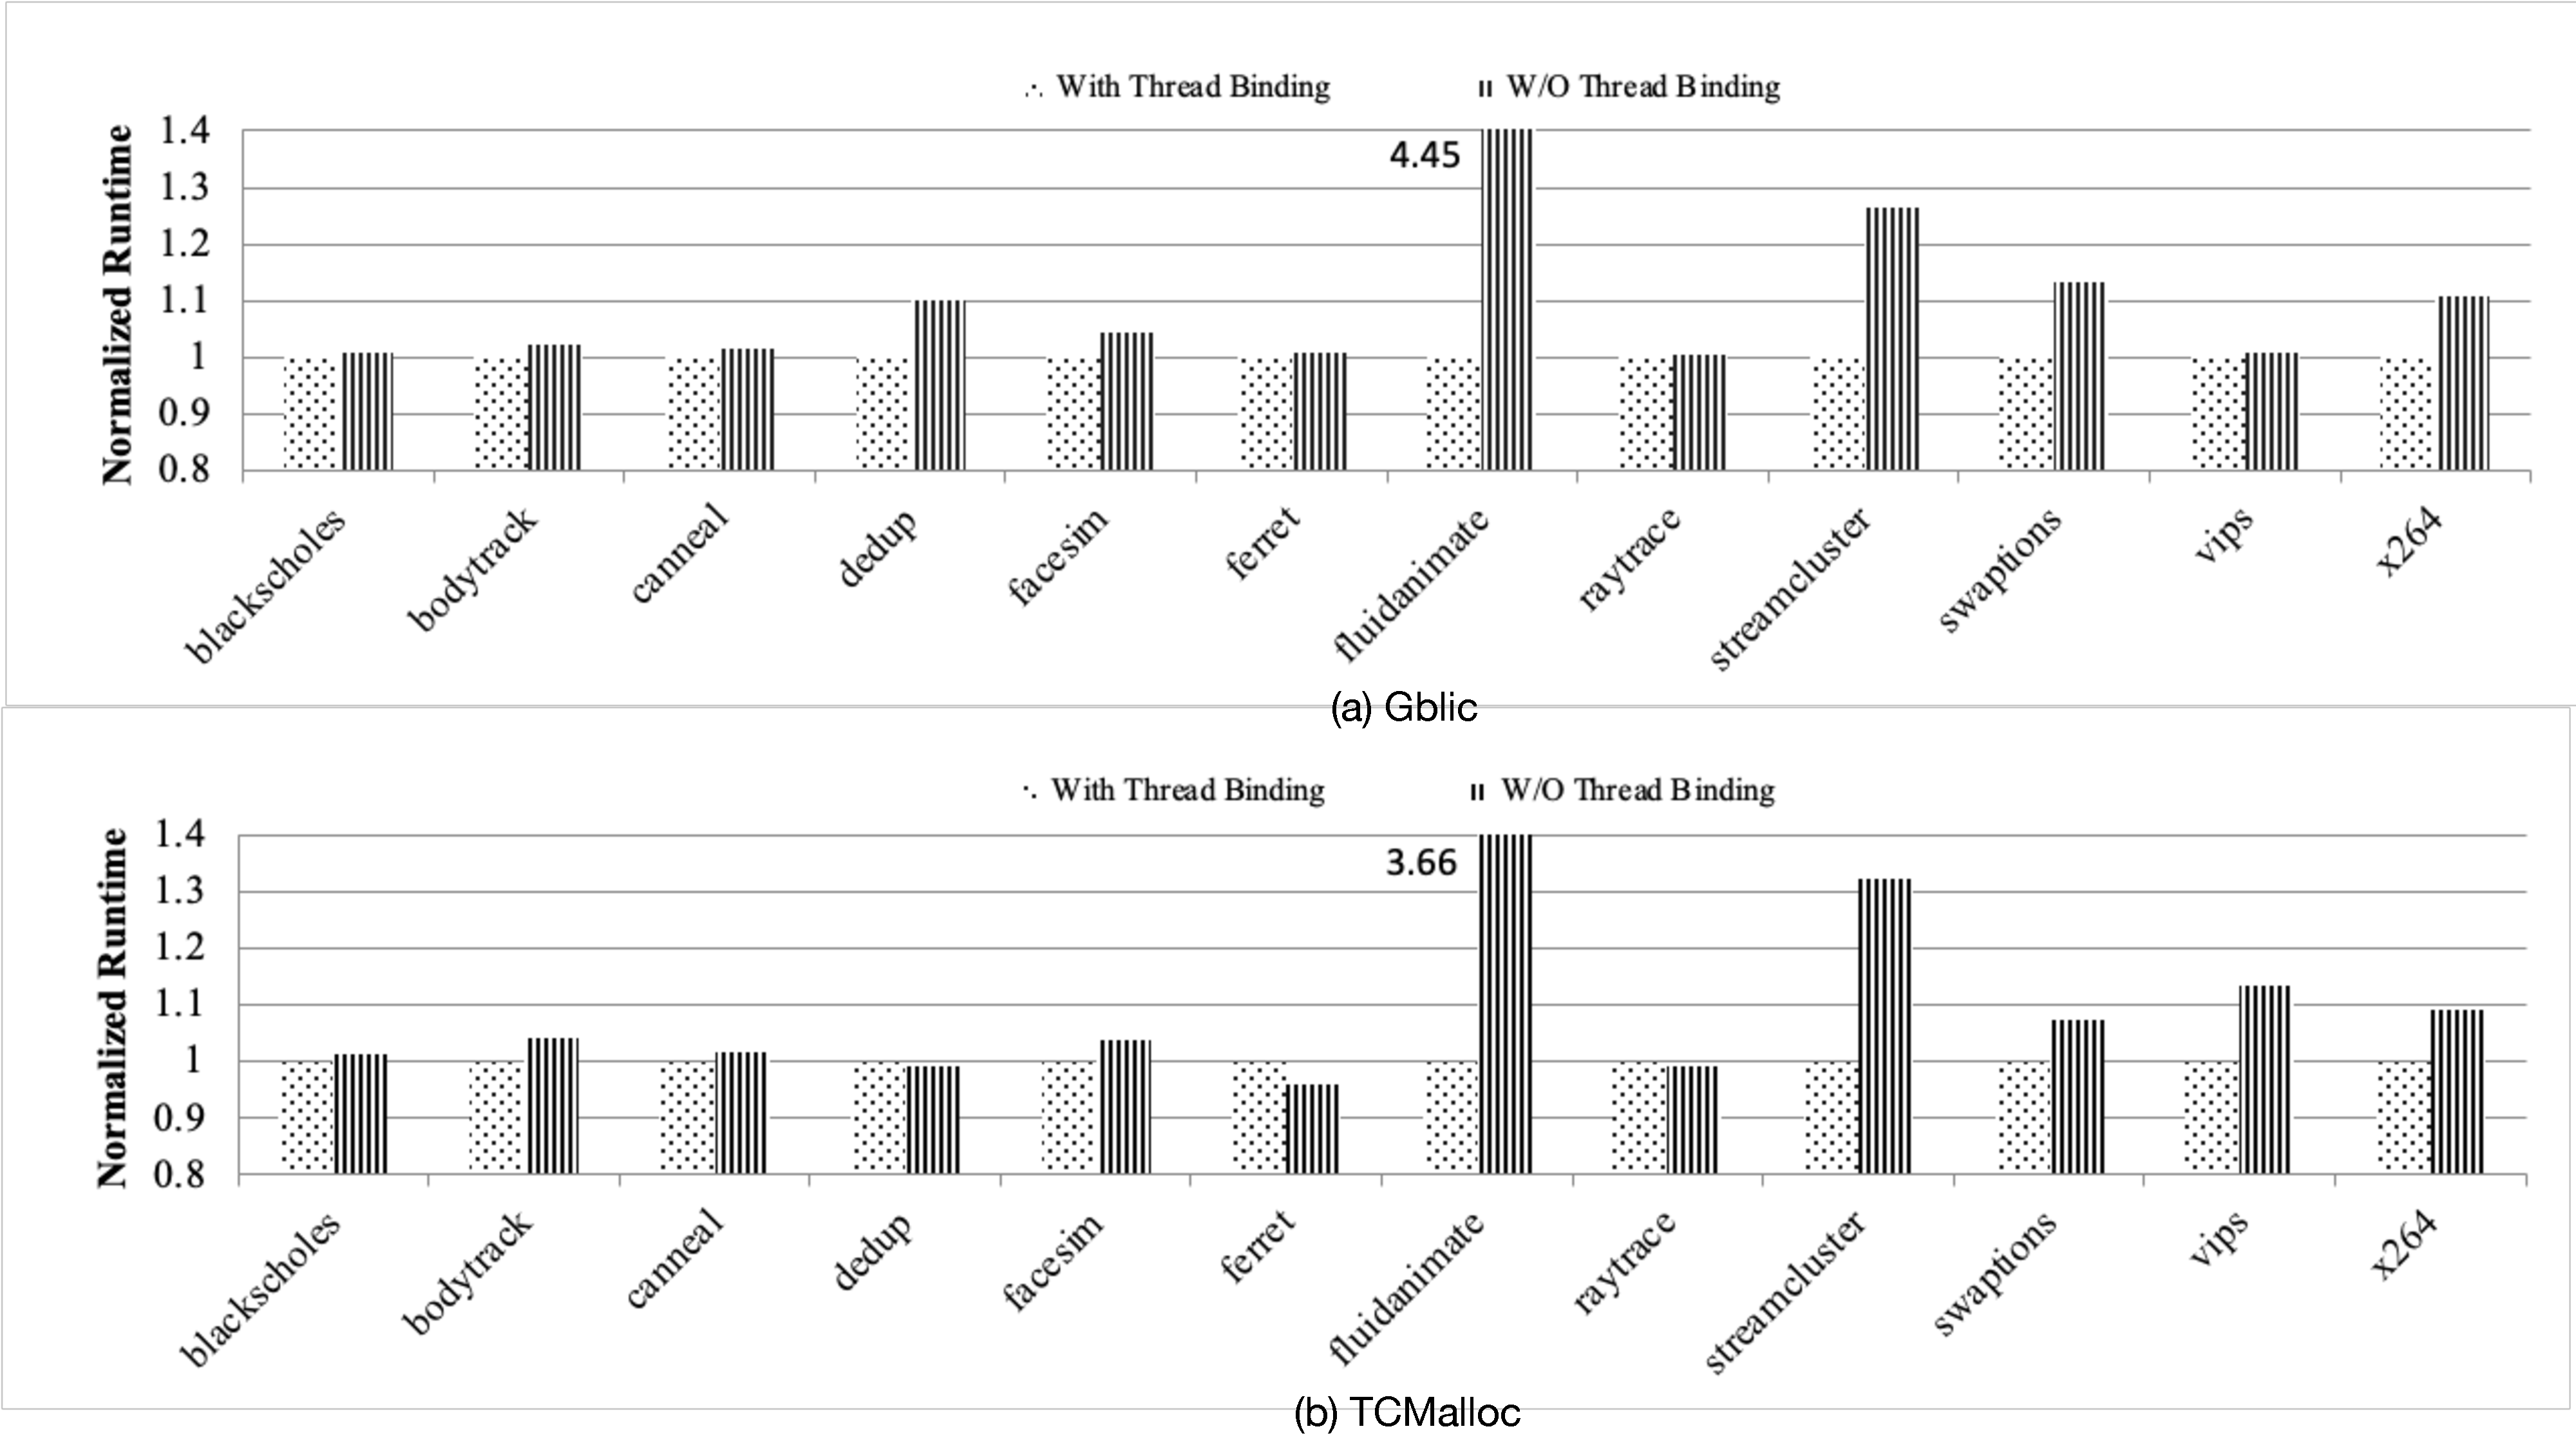
\includegraphics[width=5in]{figure/WO-pthread-binding-new2.pdf}
%    \caption{Normalized runtime with and without node-balanced thread binding for Glibc and TCMalloc.} 
%    \label{binding-pthread-scalibity}
%\end{figure*}

\begin{figure*}[!h]
\centering
\subfloat[glibc]{
   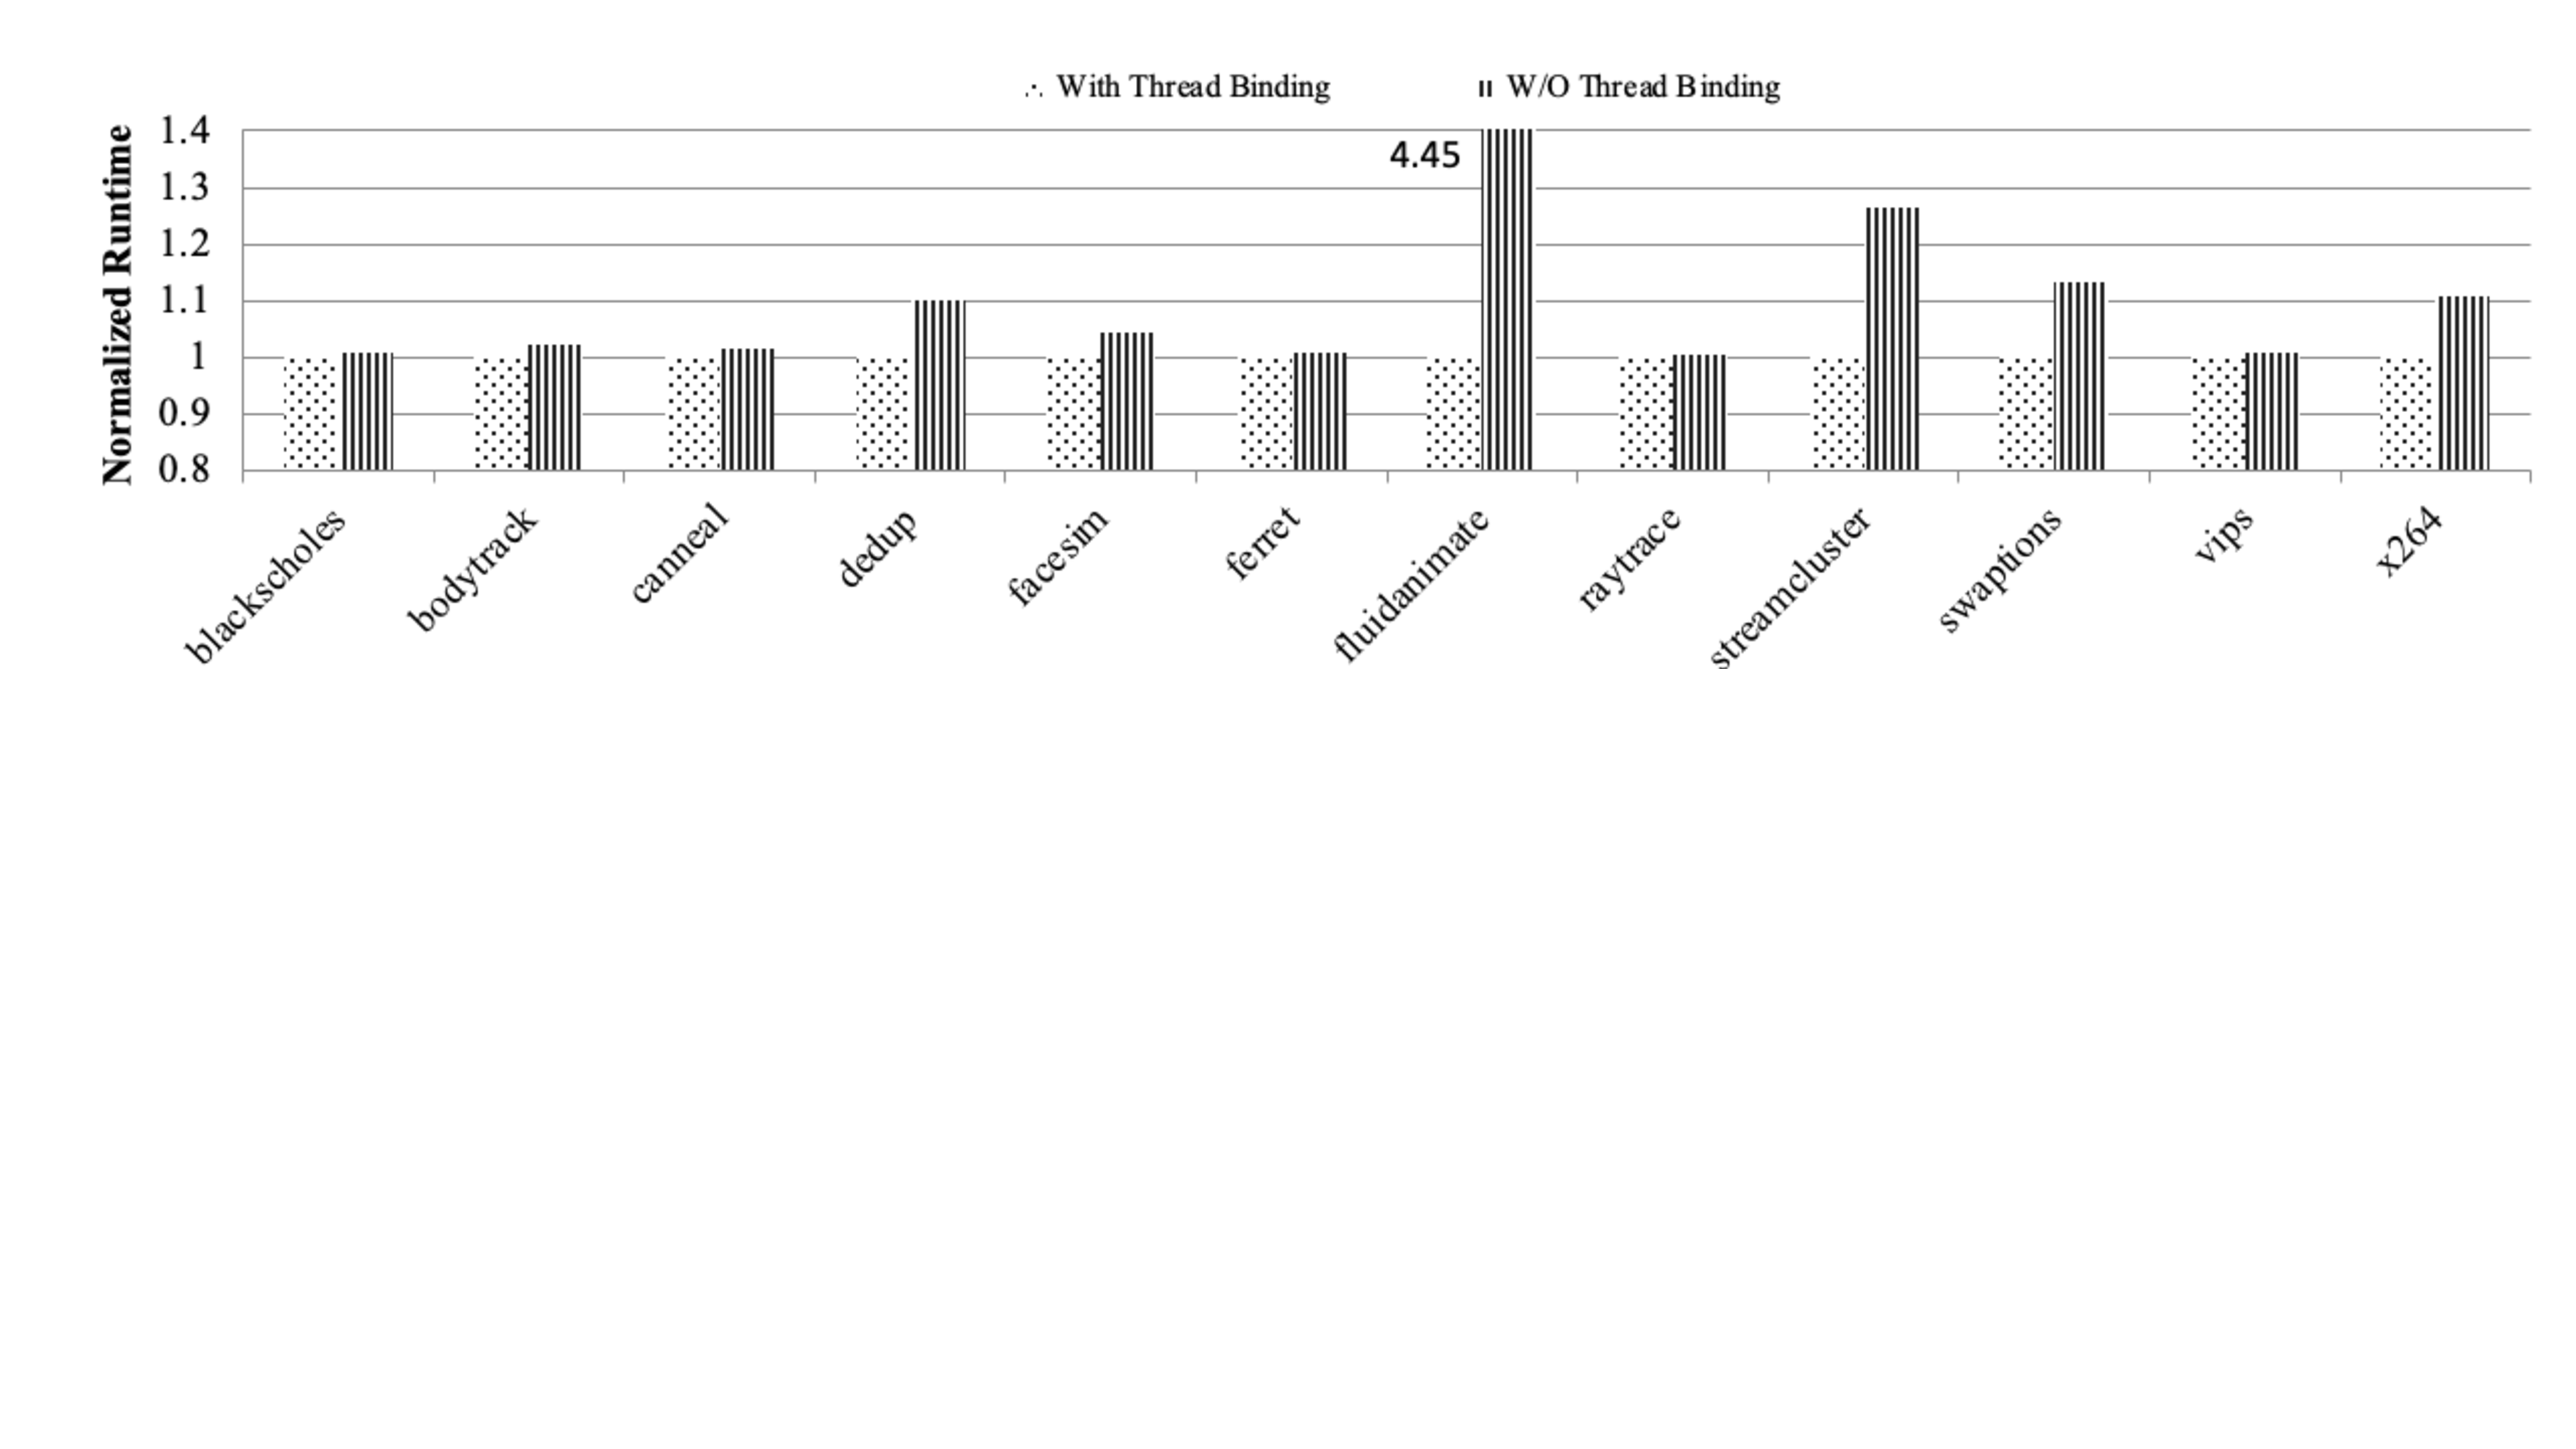
\includegraphics[width=5.5in]{figure/binding-glibc.pdf}
}

\subfloat[TCMalloc]{
   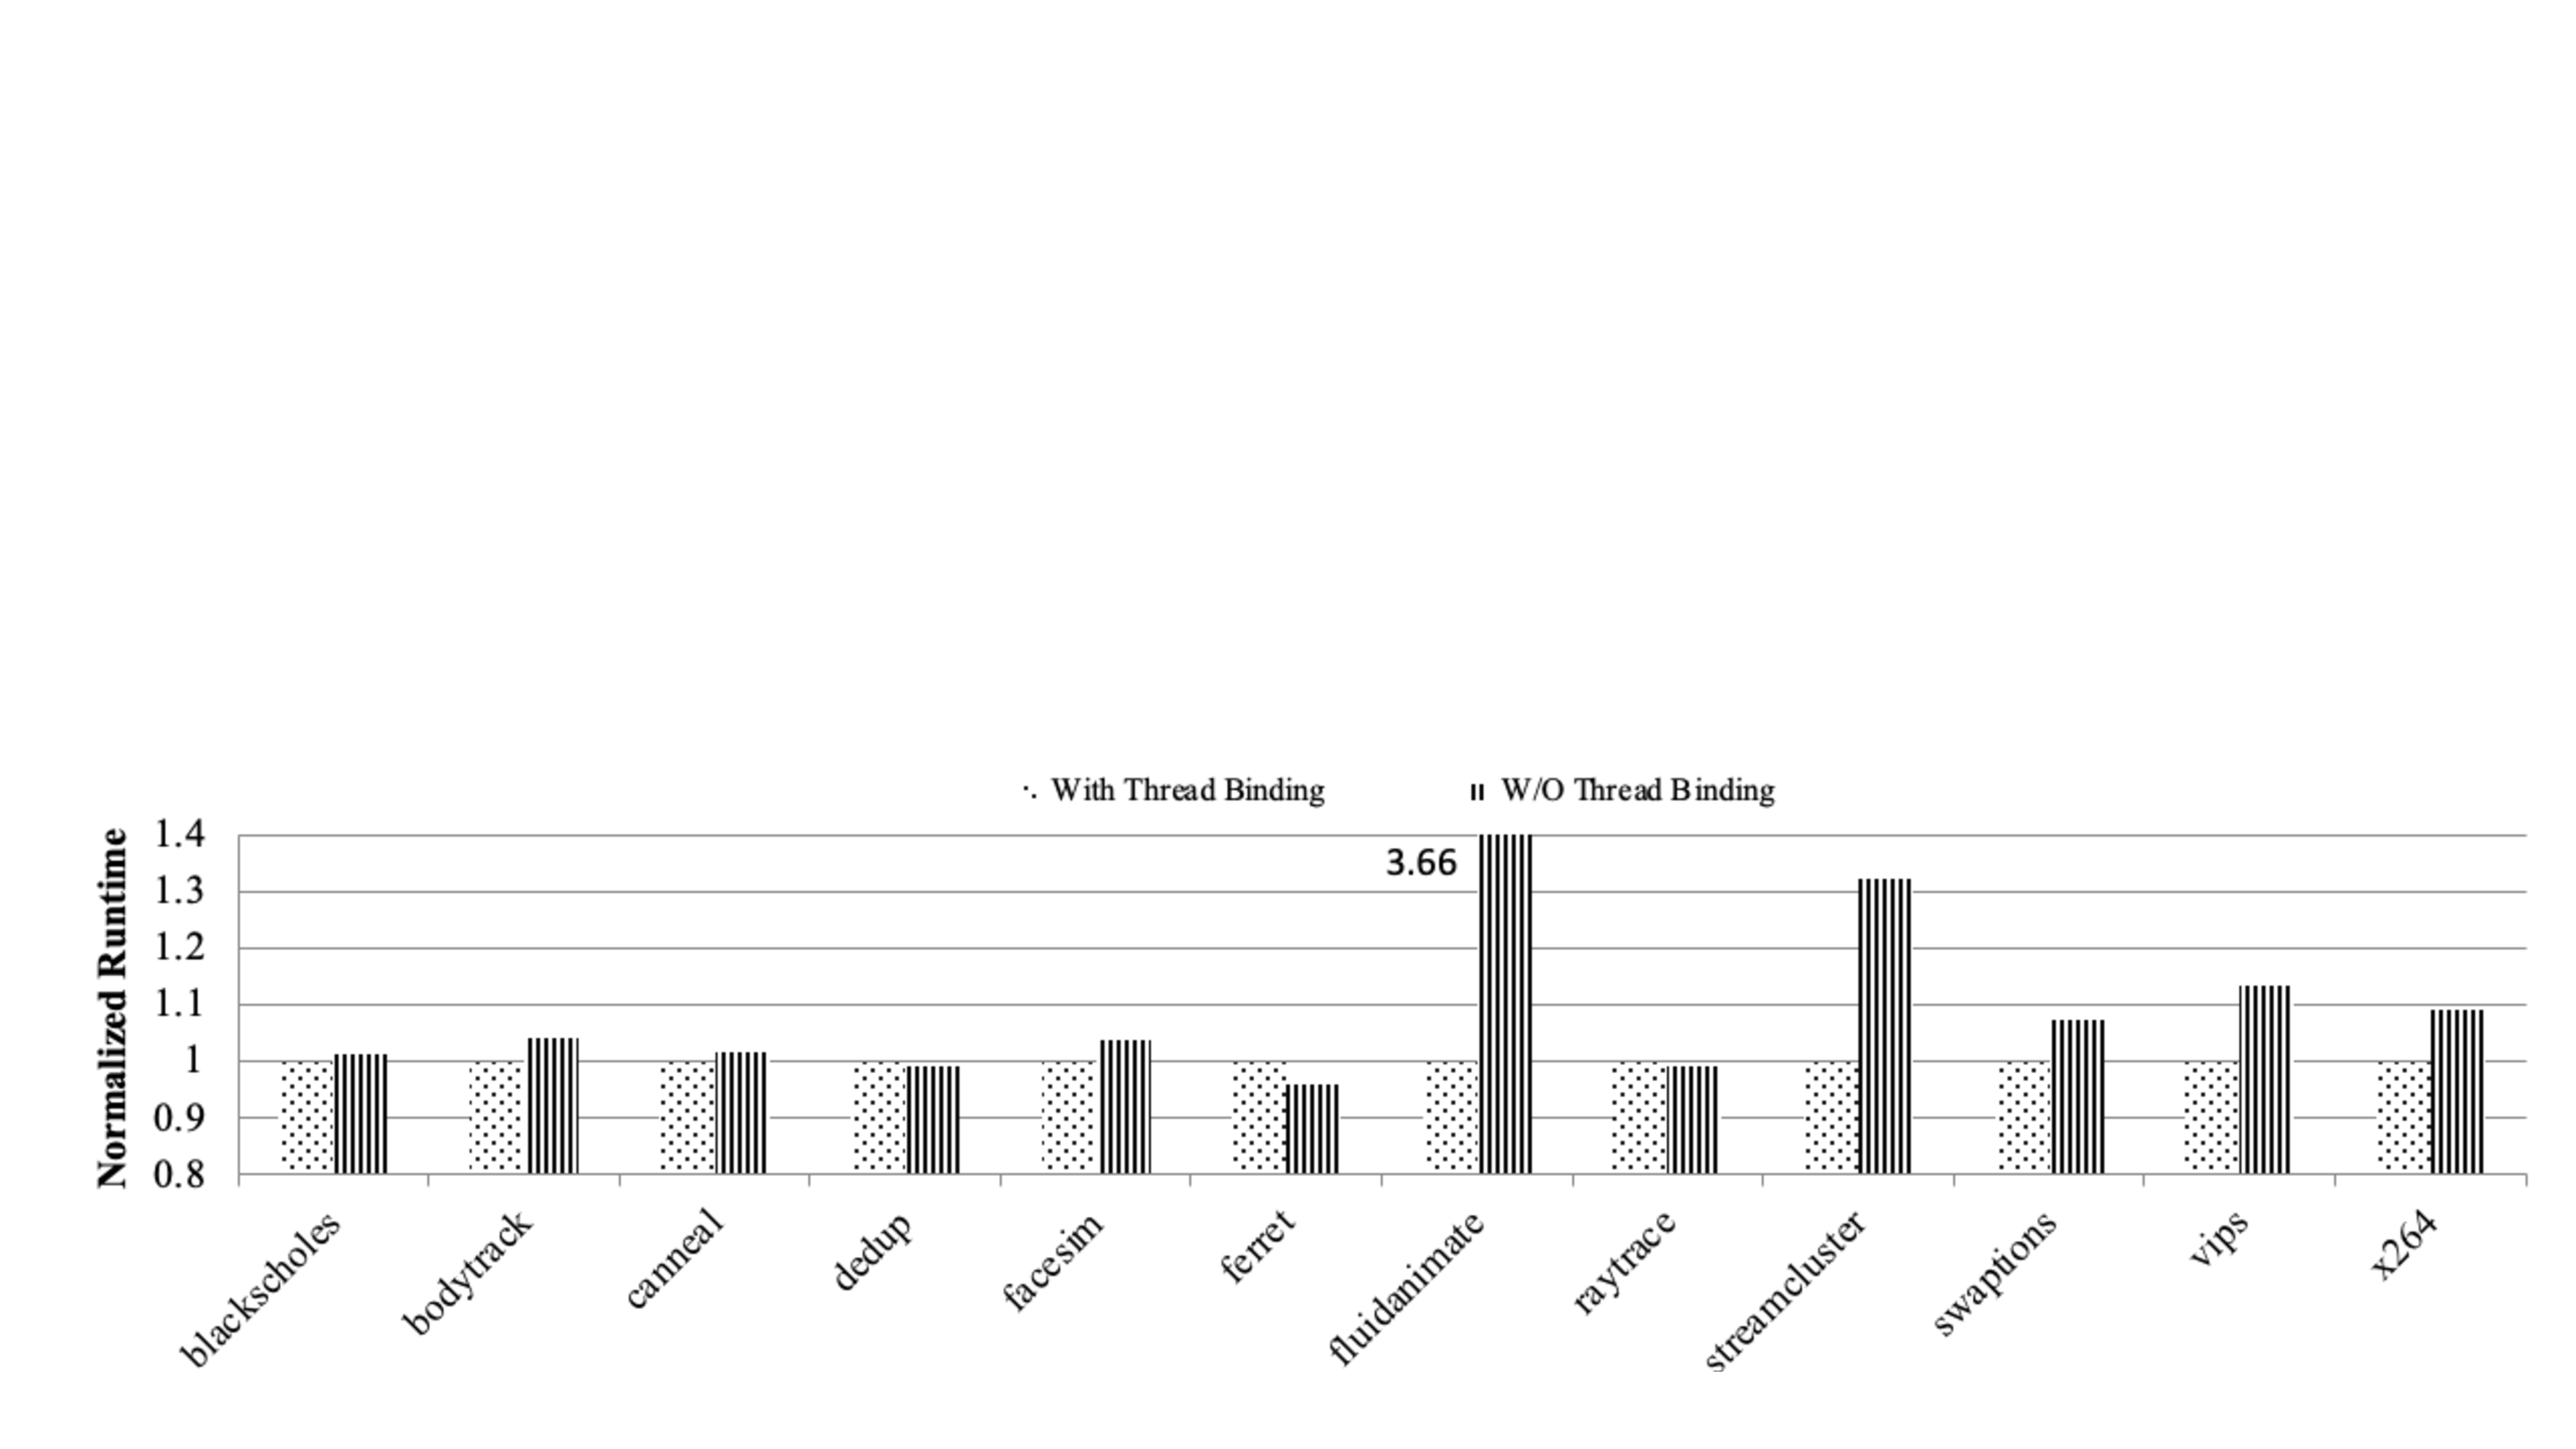
\includegraphics[width=5.5in]{figure/binding-tcmalloc.pdf}
}
\caption{Normalized runtime with and without node-balanced thread binding for Glibc and TCMalloc.}
\label{binding-pthread-scalibity}
\end{figure*}

\begin{figure*}[!ht]
    \centering
    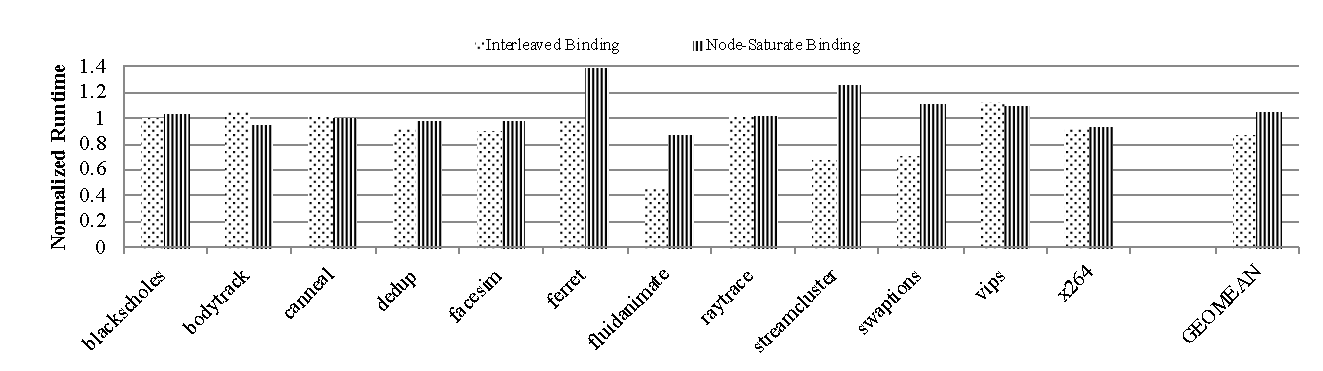
\includegraphics[width=5.5in]{figure/binding-policy.pdf}
    \caption{ Node-Balanced vs. Node-Saturate binding for Glibc, where results are normalized to those without binding.}
    \label{fig:binding-policy}  
\end{figure*}

%\todo{someone argued that the figure is so small}

Fig.~\ref{binding-pthread-scalibity} shows the performance difference with and without thread binding for two allocators, Glibc and TCMalloc. We did not evaluate \NM{} directly, since \NM{}'s mechanism is tighten to thread binding, such as its origin-based memory management, metadata allocation. In particular, threads are bound to different nodes in a round-bin way, called as node-balanced binding, which is the same as \NM{}. We observe that the thread binding improves the performance significantly for some applications. With the thread binding, \texttt{fluidanimate} runs around $4.5\times$ faster on Glibc and $3.66\times$ faster on TCMalloc. \texttt{streamcluster} runs more than 20\% and 30\% faster than the one without the binding. This clearly indicates that the thread binding will benefit the performance overall, which should be included into the memory allocator by default. 

We further  compare the Node-Balanced thread binding with Node-Saturated thread binding, which binds the maximum possible number of threads to a node and then switches to the next node. As shown in Fig.~\ref{fig:binding-policy}, the Node-Balanced thread binding is better than Node-Saturated thread binding. 

% , proving the effectiveness of Node-Balanced thread binding.

%\todo{The first figure should be Glibc}

\subsubsection{Interleaved Heap} 
\label{sec:interleavedheap}

\begin{figure*}[!ht]
    \centering
    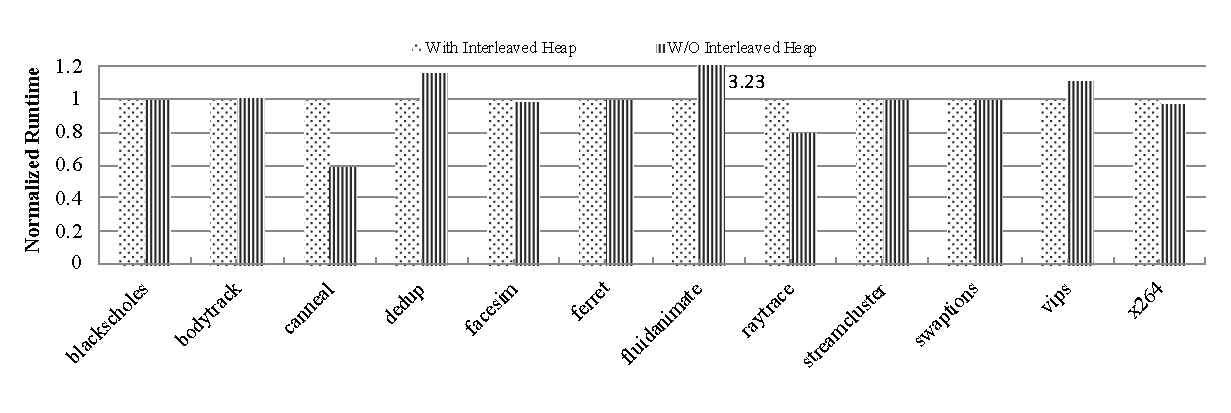
\includegraphics[width=5.5in]{figure/interleavedheap.pdf}
    \caption{Normalized runtime with and without the interleaved heap for \NM{}.  \label{fig:interleavedheap}}  
\end{figure*}


%\todo{someone argued that the figure is so small}

We also evaluate the potential benefit of the interleaved heap. The performance data is shown in Figure~\ref{fig:interleavedheap}. Note that we have evaluated all PARSEC applications listed in Section~\ref{sec:performance}.
From Figure~\ref{fig:interleavedheap}, we have the following conclusion: the interleaved heap will benefit (or at least has no harmful impact on) the performance for most applications. Some applications, such as \texttt{fluidanimate}, will have the performance speedup of $3.23\times$ with the interleaved heap. However, applications having a large portion of time spent in the serial phase, such as \texttt{canneal} and \texttt{raytrace}, may not have good performance with the interleaved heap support. 
We investigated the underlying reason for this. With the interleaved heap, \NM{} allocates the memory from all nodes in an interleaved way, instead of from the local node (based on the default first-touch policy). Therefore, some private objects that are allocated in a remote node may introduce unnecessary overhead due to remote access. Further, upon each allocation, \NM{}  checks the callstack to confirm whether an allocation is from a potentially shared heap, which also introduces some overhead. Therefore, the interleaved heap will be enabled by default, unless programmers know that it will not benefit the performance.

A simple metric is to use the portion of the serial phase inside multithreaded applications.  Programmers may turn off the interleaved heap for applications that are mostly running in serial phases.  hat is, the interleaved heap will harm the serial execution, but may benefit the parallel execution because of its load balance. It is easy to turn on/off the interleaved heap via a compilation flag or the environment variable.  

%, except applications with a large portion of serial phase (e.g., \texttt{canneal} and \texttt{raytrace})

%The interleaved heap could be utilized to avoid load imbalance issue for shared objets. 

%However, there are two issues for the interleaved heap. First, the allocator may not know whether an object is shared or not at the first time. Therefore, all objects that are allocated in the main heap (before creating any child thread) will be treated as the shared heap. Second, some applications are spending too much time in the serial phase, where the interleaved heap cannot benefit the performance for the serial phase. 





%figure ~\ref{parsec-no-interleaved-perf} we show some performance results of some applications that got significant different values after we shut down interleaved heap for \NM{}. We can see that for some applicatios with less data sharing between threads like ratrace and canneal, \NM{} could got significant improvements due to its low overheads and proper memory management. But for some other applications with intensive memory operations and sharing like fluidanimate, shutting down interleaved heap could hurt performance, since interleaved heap could help to distributed resource contention evenly over multi-nodes and then got low overheads.

%\subsubsection{Selective Huge Pages} 
%\label{sec:hugepage}

%Since the machine utilizes transparent huge pages by default, we evaluate the performance impact of huge page support on another machine with 2 NUMA-node, without enabling the transparent huge pages.
% A, the 2-node machine. We only utilize PARSEC applications for this evaluation. 

%\begin{figure}[!h]
%    \centering
%    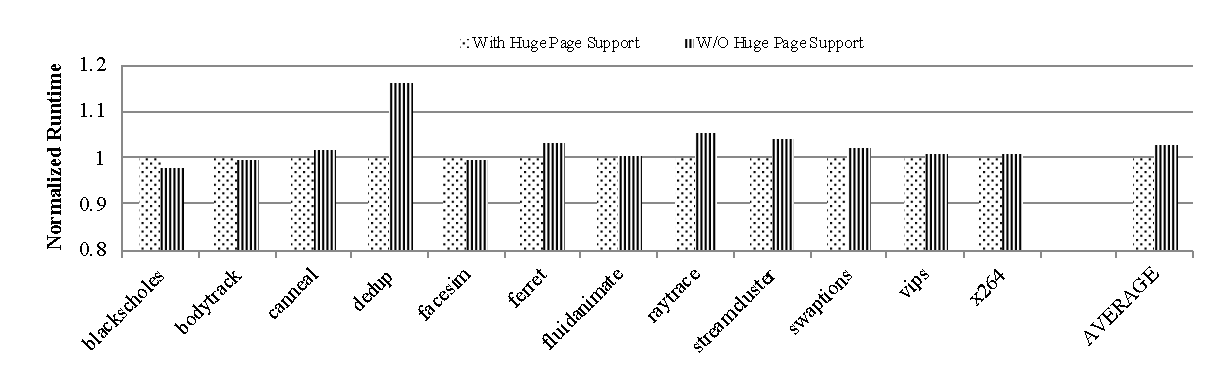
\includegraphics[width=3.2in]{figure/hugepage.pdf}
%    \caption{Normalized runtime with and without selective huge pages.}
%    \label{fig:hugepage}
%\end{figure}

%The results are shown in Figure~\ref{fig:hugepage}. When integrating with selective huge pages, \NM{} achieves a significantly better performance for \texttt{dedup}, where the performance difference is around 15\%. On average, the selective huge pages improves the performance of all evaluated applications about 2.5\%, and will not hurt the performance. This clearly indicates that it is beneficial to have selective huge pages for the NUMA architecture, especially given the fact of increasing memory size of hardware trend.  



\section{Limitation}
\label{sec:limit}

This section describes some limitations of \NM{}. First, \NM{} may consume more memory than some popular allocators, especially when transparent huge pages are enabled. \NM{} currently allocates a big chunk (larger than a huge page) from the OS, then the OS will satisfy the memory allocations with huge pages when transparent huge pages are enabled. Although this method reduces the possible system call overhead and enjoys the performance benefits caused by reducing TLB misses, it does introduce more memory consumption. That is, the whole huge page will be wasted even if applications only use a small portion in such as huge pages. However, we believe that this shortcoming is tolerable, when memory is not the major concern. 
%As shown in Figure~\ref{fig:remoteAccess}, \NM{} significantly reduces the number of TLB misses by trading with medium memory consumption. 


Second, \NM{}'s interleaved heap cannot always achieve the performance improvement due to the following reasons: (1) although the interleaved heap may avoid memory controller congestion caused by concurrent accesses from multiple child threads, it introduces unnecessary overhead for the initial thread since it is forced to have some remote accesses. (2) Although \NM{} avoids the change of programs to utilize the interleaved heap, it imposes additional overhead to identify the callsites for potentially shared objects. Therefore, users should decide whether to enable the interleaved heap or not. However, this is an easy task, since the interleaved heap may have a harmful impact when the serial phase is a big portion of the execution. Therefore, we think that this shortcoming is totally acceptable given its predictability. 

\NM{} is built based on the thread binding, where people may worry about its conflict with the OS scheduler. In fact, based on our understanding, this should not be a big issue due to the following reasons. First, \NM{}'s thread binding does not exclude OS's scheduling, as it only binds a thread to the node number. Second, \NM{} allows users to adjust the binding flexibly, although currently \NM{} only supports node-interleaved and node-saturate binding. But adding more flexible binding will be just pure engineering effort. Third, the thread binding is even suitable for server applications with thousands of threads, as \NM{}'s binding balances among different physical nodes. 
%Based on our analysis, the memory consumption is caused by \NM{}'s bag mechanism, especially with transparent huge page support. Currently, \NM{} employs one MB as a bag, which indicates that objects of each size will occupy at least of 1 MB, when transparent huge page support is enabled. Further, \NM{}'s design achieves a fast lookup on the metadata, but will utilize more memory unfortunately. We will investigate whether reducing the size of a bag could help reduce the memory consumption in the future.

%The second limitation is that \NM{} will crash less often by preallocating a huge chunk of memory from the OS in the beginning. If an invalid reference is landed within a pre-allocated range, a program will not crash, different from other allocators. Instead, \NM{} aims to achieve the high performance over the reliability. Therefore, we believe that this limitation is acceptable.  
\begin{comment}
\todo{NUMAalloc may not suitable for the situation for the system has thousands of threads. But maybe still okay, as these threads are balanced distributed to different nodes.

NUMAlloc can be useful for certain applications and system configurations and appears to be well-crafted. 

Maybe we could say that numa support is a daunting task, but it is actually not. This paper shows how to use and embedded these mechanisms in order to choose a better result. 
Interleaving shared objects similarly can make sense (e.g. as in the applications used in the evaluation of the paper) but is not easy to accept that it will universally work well or better than other techniques. As a different case from the one above, consider a server where tens-hundreds of different applications are running, possibly in containers/VMs, starting and finishing dynamically. What does interleaving shared objects say for such cases?

}

\end{comment}

\section{Related Work}

\label{sec:related}

This section discusses some related work with \NM{}. 

\paragraph{General Purpose Allocators}
 There exists a large number of allocators~\cite{dlmalloc,Hoard,tcmalloc,jemalloc,Scalloc}, but they are not designed for the NUMA architecture. Based on the management of small objects, allocators can be further classified into multiple types, such as sequential, BiBOP, and region-based allocators~\cite{Gay:1998:MME:277650.277748,  DieHarder}. Region-based allocators are suitable for special situations where all allocated objects within the same region can be deallocated at once~\cite{Gay:1998:MME:277650.277748}. For sequential allocators, subsequent memory allocations are satisfied in the continuous memory area, such as the Linux allocator~\cite{dlmalloc} and Windows allocator~\cite{DieHarder}. That is, objects of different sizes can be placed continuously. For BiBOP-style allocators, one or multiple continuous pages are treated as a ``bag'', holding objects with the same size class. \NM{} also belongs to BiBOP-style allocators, as do many other high-performance and security-focused allocators ~\cite{tcmalloc, jemalloc, Hoard, Scalloc, DieHarder}. But \NM{}
  proposes multiple special designs for the NUMA architecture.
 
 %\todo{Adding supermalloc and mimalloc}

\paragraph{NUMA-aware Allocators} TCMalloc-NUMA adds additional node-based freelists and free spans to store freed objects and pages belonging to the same node~\cite{tcmallocnew}, which is similar to \NM{}. It also invokes the \texttt{mbind} system call to bind physical memory allocations to the node that the current thread is running on, which is similar to JArena~\cite{yang2019jarena}. But JArena requires the co-design of applications, runtime system and the underlying OS, which is not transparent to users~\cite{yang2019jarena}. Also, both of them do not support the interleaved heap, invokes too many \texttt{mbind} system calls, and does not handle the metadata's locality. nMART proposes a NUMA-aware memory allocation for soft real-time system~\cite{kim2013node}. It proposes a node-oriented allocation policy to minimize the access latency, and ensures temporal and spatial guarantee for real-time systems. nMART requires the change of the underlying OS, which is different from \NM{}. nMART also has a different target as \NM{} that tries to meet the time requirement of real-time systems, and \NM{} focuses more on the performance. mimalloc also supports NUMA memory management~\cite{mimalloc}. It records the associated numa node for each segment, and tries to obtain a segment from the same node when reusing segments between threads. However, mimalloc cannot ensure local alloctions when a thread is migrated. \NM{} overcomes these issues, and further balance the memory accesses from different nodes via its node-balanced thread binding and interleaved heap. 


\paragraph{NUMA-Aware Java Heap Management} Some approaches that focus on improving the performance of Java applications, but they are not general purpose memory allocators. Ogasawara et al. focus on finding the preferred node location for JAVA objects during the garbage collection and memory allocations~\cite{Ogasawara:2009:NMM:1640089.1640117}, via thread stack, synchronization information, and object reference graph. Tikir et al. propose to employ hardware performance counters to collect the runtime information of Java applications, and then migrate an object to the closet node with most accesses~\cite{1419934}. 
NumaGiC reduces remote accesses in garbage collection phases with a mostly distributed design so that each GC thread will mostly collect memory references locally, and utilize a work-stealing mode only when no local references are available~\cite{NumaGiC}.


\paragraph{Combination of Task Scheduling and Memory Management:} Redline integrates task scheduling and memory management inside the OS level~\cite{Redline}, to support interactive applications. 
Majo et al. propose to consider both data locality and cache contention to achieve better performance for the NUMA applications~\cite{Majo:2011:MMN:1993478.1993481}. Wagle observed that dynamic memory allocations, thread placement and scheduling, memory placement policies, OS configurations may help improve the query performance of in-memory databases~\cite{wagle2015numa}.  Majo et al. propose to set task-to-thread affinity, and pin threads to specific cores to achieve a better performance~\cite{Majo:2015:LPC:2688500.2688509}. Diener proposes a new kernel framework to combine task management and memory management together to achieve better performance~\cite{diener2015automatic}. 
Debes et al. propose the combination of enhanced work-pushing and deferred allocation together to improve the performance for data-parallel tasks, but focusing on special programming models~\cite{DBLP:conf/IEEEpact/DrebesPH0D16}. They inspire \NM{}'s binding-based memory management. But \NM{} is the first work that combines both together inside a memory allocator. 



\paragraph{NUMA Libraries:}
Cantalupo et al. propose multiple APIs that allow users to manage their memory in fine granularity by combining with multiple existing system calls~\cite{cantalupo2015memkind}. However, they are not targeting a general purpose allocator, since it requires programmers to manage the memory explicitly.  Majo et al. propose multiple source-code based  algorithmic changes in order to improve data sharing and memory access patterns for NUMA architectures~\cite{6704666}. Williams et al. propose to group data structures that can be migrated together with arenas~\cite{WilliamsI0L18}. 
Shoal also proposes a set of APIs that allow the user to specify memory access patterns~\cite{Kaestle:2015:SSA:2813767.2813787}. 
%Then it could automatically replicate or distribute the memory to different NUMA nodes automatically. 
But both of them need significant manual effort to employ this. 
%XPV extends virtualization technique by considering NUMA-topology and extending virtualization to SRLs ~\cite{Bui:2019:EPV:3302424.3303960}.

%\todo{Changing the following two paragraphs}
\paragraph{Reactive Systems for NUMA Architecture:} Some systems migrate tasks or physical pages reactively based on memory access patterns or other hardware characteristics~\cite{Blagodurov:2011:CNC:2002181.2002182, AutoNUMA, Dashti:2013:TMH:2451116.2451157, Lepers:2015:TMP:2813767.2813788}. 
%They improve the performance automatically without human involvement. However, these systems impose additional overhead (sometimes unnecessarily)  by migrating tasks or physical pages reactively. Further, a reactive approach cannot reduce remote accesses by the migration, if objects of the same page are concurrently accessed by multiple threads in multiple nodes~\cite{Gaud:2014:LPM:2643634.2643659}. 
\NM{} belongs to a proactive approach that does not require explicit and page migration, which is complementary to these reactive systems. 
%It is possible to combine these two together to achieve better performance. 

%The second approach relies on programmers to manage memory allocations and task assignments explicitly~\cite{Kaestle:2015:SSA:2813767.2813787, Lin:2016:MTP:2872362.2872401, Majo:2017:LPC:3057718.3040222}. Although they could improve the performance greatly, they typically require significant human effort to rewrite the programs, where legacy systems cannot benefit automatically. 

\section{Conclusion}
\label{sec:conclusion}

\NM{} is a memory allocator that is specially designed for the NUMA architecture. Applications can be linked to \NM{} directly, without the change of code and the recompilation. \NM{} is different from existing memory allocators, since it proposes fine-grained memory management to accommodate the heterogeneity of both modern hardware and applications. It further proposes origin-based allocations to improve the locality, node-balanced thread binding and an interleaved heap to reduce the load imbalance, and explicit huge pages to employ the benefits of huge pages. 
Based on our extensive evaluation, \NM{} achieves a significantly better performance than other popular allocators on the NUMA architecture, with 16.4\% performance speedup on average and up to $6.4\times$ faster.
%\NM{} is available at https://github.com/XXX. 

\bibliographystyle{IEEEtranS}
\bibliography{ref,emery,tongping}

\end{document}
